\chapter{Analisi cinematica dei meccanismi piani}

	
		Le catene cinematiche sono lo scheletro da cui ogni meccanismo nasce. Tra le molteplici catene cinematiche che si possono trovare e immaginare una fondamentale distinzione va fatta  prima di proseguire con la loro trattazione: catene cinematiche a catena chiusa e a catena aperta.
		
		Per quanto elementare tale distinzione possa essere, non altrettanto elementare è la loro analisi cinematica: infatti, molte macchine, come, a titolo di esempio, i \textbf{manipolatori}, prevedono la connessione di membri secondo uno schema a catena cinematica (sia essa aperta o chiusa) e il conseguente controllo dei molteplici G.d.L. che gli possono essere attribuiti può, a volte, risultare problematico. (Soprattutto qualora si voglia posizionare un organo di tale macchina nello spazio)
		
		Procediamo, dunque, alle modalità di analisi dei meccanismi piani in catena aperta e chiusa.
		\section{Analisi cinematica dei meccanismi piani in catena aperta}
			
			\begin{minipage}{.5\textwidth}
				Consideriamo un sistema piano in catena aperta di cui vogliamo conoscere posizione, velocità ed accelerazione dei vari punti appartenenti ai membri del corpo.
			
			Come esempio consideriamo un escavatore con i cingoli bloccati: è un meccanismo in catena aperta formato da tre membri rigidi (\emph{uno è a telaio}) connessi da 2 coppie rotoidali $c_1$.
			\end{minipage}
			\hfill
			\begin{minipage}{.5\textwidth}
				\centering
				\includegraphics[width = .8\textwidth]{chapter03/Immagine44}
			\end{minipage}
			\vspace{1mm}
			
			Dalla figura dell'escavatore sopra proposta e dall'eventuale analisi del meccanismo, possiamo notare che tale sistema di corpi prevede 4 G.d.L. attribuibili a:
			\begin{itemize}
				\item Rotazione intorno all'asse verticale
				\item Movimento di sollevamento del braccio
				\item Controllo del movimento dell'articolazione del gomito
				\item Controllo del movimento del polso
			\end{itemize}
			
			Per ora, come già accennato ad inizio capitolo, ci soffermeremo sull'analisi cinematica dei meccanismi piani, dove, di conseguenza, non è prevista la rotazione intorno all'asse verticale.
			
			Il meccanismo così descritto presenta 3 G.d.L. che possono essere facilmente individuati nel controllo dei 3 attuatori in figura.
			
			Per ragioni di semplificazione dei calcoli analitici, che tuttavia non compromettono la spiegazione delle modalità di analisi che andremo ad esporre in questa sezione, ci poniamo l'obiettivo di descrivere la posizione, la velocità e l'accelerazione del punto P (in corrispondenza del collegamento tramite coppia R tra il sistema 2 e la benna).
			 
			 In tal modo priviamo la nostra analisi dello studio di un ulteriore G.d.L. (attribuibile alla posizione della benna stessa): il punto P, infatti, risulta un punto solidale al sistema 2 (le sue coordinate rispetto ad un sistema di riferimento solidale a sistema 2 sono, cioè, costanti).
			 
			 Hic rebus stantibus procediamo alla descrizione del meccanismo in questione.
			 
			 \begin{enumerate}
			 	\item Il punto P è solidale al sistema di riferimento 2 (a cui faremo riferimento con il termine \emph{sistema 2}).
			 		Ciò, come già indicato in precedenza, comporta che le coordinate del punto P rispetto a tale sistema siano costanti.
			 		
			 		Tali coordinate verranno identificate dalla notazione: \hspace{3mm} $\leftidx{^2}{\begin{Bmatrix} x_P\\y_P\end{Bmatrix}}$
				\item Si consideri un secondo sistema di riferimento, solidale al corpo 1 (tra telaio e corpo 2) (a cui faremo riferimento con il termine \emph{sistema 1}).
				
				La proiezione delle coordinate del punto P sul sistema di riferimento 1 prevedono l'utilizzo della relativa matrice di rotazione e assume la seguente forma:
				\begin{equation*}
					\leftidx{^1}{\begin{Bmatrix}x_P\\y_P\end{Bmatrix}} =
					\leftidx{^1}{\begin{Bmatrix}x_{O2}\\y_{O2}\end{Bmatrix}}\,+\,
					\leftidx{^1_2}{\begin{bmatrix}R\end{bmatrix}}\quad
					\leftidx{^2}{\begin{Bmatrix}x_P\\y_P\end{Bmatrix}}
				\end{equation*}
				
				\item Infine, per esplicitare le coordinate del punto P e il relativo moto, si consideri l'introduzione di un ultimo sistema di riferimento fisso.
					Allo stesso modo del punto precedente le coordinate del punto P rispetto a tale sistema di riferimento risultano essere:
					
					\begin{align*}
						\leftidx{^f}{\begin{Bmatrix}x_P\\y_P\end{Bmatrix}} &= 
						\leftidx{^f}{\begin{Bmatrix}x_{O1}\\y_{O1}\end{Bmatrix}}\,+\,
						\leftidx{^f_1}{\begin{bmatrix}R\end{bmatrix}}\,\,
						\leftidx{^1}{\begin{Bmatrix}x_P\\y_P\end{Bmatrix}}\\
						&= \leftidx{^f}{\begin{Bmatrix}x_{O1}\\y_{O1}\end{Bmatrix}}\,+\,
						\leftidx{^f_1}{\begin{bmatrix}R\end{bmatrix}}\,\,
						\leftidx{^1}{\begin{Bmatrix}x_{O2}\\y_{O2}\end{Bmatrix}}\,+\,
						\leftidx{^f_1}{\begin{bmatrix}R\end{bmatrix}}\,
						\leftidx{^1_2}{\begin{bmatrix}R\end{bmatrix}}\,
						\leftidx{^2}{\begin{Bmatrix}x_{P}\\y_{P}\end{Bmatrix}}		\quad//\emph{sostituzione dell'espressione al punto 2}\\
						&=  \leftidx{^f}{\begin{Bmatrix}x_{O1}\\y_{O1}\end{Bmatrix}}\,+\,
						\leftidx{^f_1}{\begin{bmatrix}R\end{bmatrix}}\,\,
						\leftidx{^1}{\begin{Bmatrix}x_{O2}\\y_{O2}\end{Bmatrix}}\,+\,
						\leftidx{^f_2}{\begin{bmatrix}R\end{bmatrix}}\,
						\leftidx{^2}{\begin{Bmatrix}x_{P}\\y_{P}\end{Bmatrix}}
					\end{align*}
			 \end{enumerate}
			 \vspace{2mm}
			 
			 \begin{minipage}{.5\textwidth}
			 	\centering
			 	\includegraphics[width = .95\textwidth]{chapter03/Immagine45}
			 \end{minipage}
			 \hfill
			 \begin{minipage}{.5\textwidth}
			Una parentesi va aperta riguardo alla scelta degli angoli quando si ha a che fare con una matrice di rotazione:\newline
			
			I due principali metodi di rappresentazione coinvolgono angoli relativi e angoli assoluti, che sono rappresentati nelle figure a lato.
			
			La scelta che è stata effettuata a priori per l'analisi della cinematica dei moti della macchina in esame è la seconda. Infatti, l'utilizzo di angoli assoluti semplifica notevolmente la definizione della matrice di rotazione:
			\end{minipage}\newline
			
			\begin{enumerate}[$\rightarrow$]
				\item {\scshape{\bfseries angoli assoluti}}
					\begin{equation*}
						\leftidx{^f_1}{\begin{bmatrix}R\end{bmatrix}} = f (q_1) =
						\begin{bmatrix}
							\cos{q_1} & -\,\sin{q_1}\\
							\sin{q_1} & \cos{q_1}
						\end{bmatrix}
						\end{equation*}
						\emph{la matrice di rotazione da 1 ad f è esclusivamente funzione dell'angolo assoluto $q_1$}
						
						
						\begin{equation*}
						\leftidx{^f_2}{\begin{bmatrix}R\end{bmatrix}} = f (q_2) =
						\begin{bmatrix}
							\cos{q_2} & -\,\sin{q_2}\\
							\sin{q_2} & \cos{q_2}
						\end{bmatrix}
					\end{equation*}
					\emph{la matrice di rotazione da 2 ad f è esclusivamente funzione dell'angolo assoluto $q_2$}
				
				\item  {\scshape{\bfseries angoli relativi}}
				
					Mentre la conclusione riguardante la matrice di rotazione da 1 ad f non cambia, lo stesso non può essere detto della matrice da 2 ad f:
					
					\begin{align*}
						\leftidx{^f_2}{\begin{bmatrix}R\end{bmatrix}} &=
						\leftidx{^f_1}{\begin{bmatrix}R\end{bmatrix}}\,\,
						\leftidx{^1_2}{\begin{bmatrix}R\end{bmatrix}}\\
						&= \begin{bmatrix}
						\cos{q_1}\,\cos{q_2}\,-\,\sin{q_1}\,\sin{q_2} \quad & -\,\cos{q_1}\,\sin{q_2}\,-\,\sin{q_1}\,\cos{q_2}\\
						\sin{q_1}\,\cos{q_2}\,-\,\cos{q_1}\,\sin{q_2} \quad & \cos{q_1}\,\cos{q_2}\,-\,\sin{q_1}\,\sin{q_2}
						\end{bmatrix}\\
						&= \begin{bmatrix}
						\cos{(q_1 + q_2)} & -\,\sin{(q_1 + q_2)}\\
						\sin{(q_1 + q_2)} & \cos{(q_1 + q_2)}
						\end{bmatrix}
					\end{align*}
					
					In conclusione: possiamo ammettere che $q_{1R}\,+\,q_{2R} = q_{2A}$				
			\end{enumerate}
			 
			 
			 Continuiamo l'analisi della cinematica della nostra macchina con la cosiddetta analisi di velocità: applichiamo, dunque, le formule ottenute nel capitolo precedente anche in questo caso mantenendo la convenzione di angoli assoluti.
			 
			 \begin{equation*}
			 	\leftidx{^f}{\begin{Bmatrix}\dot{x_P}\\\dot{y_P}\end{Bmatrix}} =
			 	\leftidx{^f}{\begin{Bmatrix}\dot{x_{O1}}\\ \dot{y_{O1}}\end{Bmatrix}}\,+\,\dot{q_1}\,\,
			 	\leftidx{^f_1}{\begin{bmatrix} R \end{bmatrix}}\,
			 	\begin{bmatrix}P\end{bmatrix}\,
			 	\leftidx{^1}{\begin{Bmatrix} x_{O2}\\ y_{O2} \end{Bmatrix}}\,+\,\dot{q_2}\,\,
			 	\leftidx{^f_2}{\begin{bmatrix} R \end{bmatrix}}\,
			 	\begin{bmatrix}P\end{bmatrix}\,
			 	\leftidx{^2}{\begin{Bmatrix}x_{P}\\y_{P}\end{Bmatrix}}
			 	\end{equation*}
			 	
			\footnote{Si ricorda ancora una volta che $\leftidx{^1}{\begin{Bmatrix} x_{O2} \\ y_{O2} \end{Bmatrix}} = cost.$ e che la matrice di permutazione $\begin{bmatrix}P\end{bmatrix} = \begin{bmatrix}0 & -\,1\\ 1 & 0\end{bmatrix}$}
			
			Per concludere svolgiamo l'analisi di accelerazione:
			
			\begin{align*}
				\leftidx{^f}{\begin{Bmatrix}\ddot{x_P}\\\ddot{y_P}\end{Bmatrix}} =
				\leftidx{^f}{\begin{Bmatrix}\ddot{x_{O1}}\\\ddot{y_{O1}}\end{Bmatrix}}\,&+\,\ddot{q_1}
				\leftidx{^f_1}{\begin{bmatrix} R \end{bmatrix}}\,\,
				\begin{bmatrix}P\end{bmatrix}\,\,
				\leftidx{^1}{\begin{Bmatrix}x_{O2}\\y_{O2}\end{Bmatrix}}\,+\, \dot{q_1}^2\,\,
				\leftidx{^f_1}{\begin{bmatrix} R \end{bmatrix}}\,\,
				\M{P}\,\M{P}\,\,
				\leftidx{^1}{\begin{Bmatrix}x_{O2}\\y_{O2}\end{Bmatrix}}\\
				&+\,\,\ddot{q_2}
				\leftidx{^f_2}{\begin{bmatrix} R \end{bmatrix}}\,\,
				\begin{bmatrix}P\end{bmatrix}\,\,
				\leftidx{^2}{\begin{Bmatrix}x_{P}\\y_{P}\end{Bmatrix}}\,+\, \dot{q_2}^2\,\,
				\leftidx{^f_2}{\begin{bmatrix} R \end{bmatrix}}\,\,
				\M{P}\,\M{P}\,\,
				\leftidx{^2}{\begin{Bmatrix}x_{P}\\y_{P}\end{Bmatrix}}\\
				= 
				\leftidx{^f}{\begin{Bmatrix}\ddot{x_{O1}}\\\ddot{y_{O1}}\end{Bmatrix}}\,&+\,\ddot{q_1}
				\leftidx{^f_1}{\begin{bmatrix} R \end{bmatrix}}\,\,
				\begin{bmatrix}P\end{bmatrix}\,\,
				\leftidx{^1}{\begin{Bmatrix}x_{O2}\\y_{O2}\end{Bmatrix}}\,-\, \dot{q_1}^2\,\,
				\leftidx{^f_1}{\begin{bmatrix} R \end{bmatrix}}\,\,
				\leftidx{^1}{\begin{Bmatrix}x_{O2}\\y_{O2}\end{Bmatrix}}\\
				&+\,\,\ddot{q_2}
				\leftidx{^f_2}{\begin{bmatrix} R \end{bmatrix}}\,\,
				\begin{bmatrix}P\end{bmatrix}\,\,
				\leftidx{^2}{\begin{Bmatrix}x_{P}\\y_{P}\end{Bmatrix}}\,
				-\,\dot{q_2}^2\,\,
				\leftidx{^f_2}{\begin{bmatrix} R \end{bmatrix}}\,\,
				\leftidx{^2}{\begin{Bmatrix}x_{P}\\y_{P}\end{Bmatrix}}
			\end{align*}
			
			\footnote{Si ricorda al lettore che $\begin{bmatrix}P\end{bmatrix}\,\,\begin{bmatrix}P\end{bmatrix} = \begin{bmatrix}0&-1\\1&0\end{bmatrix}\,\, \begin{bmatrix}0&-1\\1&0\end{bmatrix} = \begin{bmatrix}-1 &0\\0&-1\end{bmatrix} = -\,\,\begin{bmatrix}1&0\\0&1\end{bmatrix}$}
			
			In cui si distinguono i termini di:
			\begin{enumerate}[£]
			\item Accelerazione dell'origine del sistema 1
			\item Accelerazione tangenziale denotata dal fattore moltiplicativo $\dot{q_i}$ 
			\item Accelerazione centripeta individuata dal fattore moltiplicativo $-\,\ddot{q_i}^2$
			\end{enumerate}
			
			Se ne deduce che nel caso di meccanismi piani l'analisi cinematica è relativamente semplice; infatti è stato agevole esprimere analiticamente le coordinate del punto P, e delle sue derivate rispetto al tempo, in forma esplicita, in funzione delle coordinate libere:
			\begin{gather*}
				x_P = \emph{f}(q_1,\,q_2,\,t)\qquad;\qquad \dot{x_P} = \emph{f}(q_1,\,q_2,\,\dot{q_1},\,\dot{q_2},\,t)\qquad;\qquad \ddot{x_P} = \emph{f}(q_1,\,q_2,\,\dot{q_1},\,\dot{q_2},\,\ddot{q_1},\,\ddot{q_2},\,t)
			\end{gather*}
			
			Per la definizione delle prestazioni e del campo di lavoro di un meccanismo piano è importante, specie per le applicazioni in cui si vuole che un certo membro raggiunga una determinata zona nello spazio, conoscere il campo ammissibile degli spostamenti nel piano dei vari membri del meccanismo, in funzione della geometria e del tipo di accoppiamenti.
			
		Si tratta quindi di studiare la mobilità del meccanismo; l'analisi di mobilità può essere svolta in due diverse modalità:
		\vspace{1mm}
		
			\begin{minipage}{.5\textwidth}	
			\begin{itemize}
				\item \textbf{Nozione semplice di spazio raggiungibile}: ovvero tutti i punti che l'organo di interesse riesce a raggiungere (\emph{cfr. escavatore})
				\item \textbf{Nozione di spazio destro}: ovvero lo spazio che l'organo di interesse può occupare (tramite rotazioni e altri moti relativi tra i membri) al raggiungimento di un determinato punto. (\emph{cfr. manipolatore industriale})
			\end{itemize}
			\end{minipage}
			\hfill
			\begin{minipage}{.5\textwidth}
			\centering
			\includegraphics[width = .95\textwidth]{chapter03/Immagine46}
			\end{minipage}
			
			\section{Analisi cinematica di meccanismi piani con una catena chiusa}
			
			Abbiamo visto che se un meccanismo ha un solo G.d.L. esso può essere descritto completamente con una sola coordinata generalizzata.
			
			Perciò il problema che si pone è il seguente: data la coordinata generalizzata e la sua derivata prima (\emph{velocità}) e la sua derivata seconda (\emph{accelerazione}) calcolare la posizione, velocità e accelerazione di tutti i punti del meccanismo.
			
			In genere questo calcolo non viene fatto per un solo valore della coordinata generalizzata e delle sue derivate, ma per tutto un insieme di valori; in sostanza si vuole studiare il movimento del meccanismo.
			
			Esistono vari metodi per risolvere tale problema, ma quello che verrà esposto in questa sezione sarà la cosiddetta: \textbf{analisi cinematica di meccanismi in catena chiusa con il poligono di chiusura}
			
			Broadly speaking se esiste una catena cinematica chiusa è possibile compiere un percorso chiuso che comprenda corpi diversi del meccanismo in esame.
			
			\subsection{Glifo oscillante}
			\begin{center}
				{\scshape{\bfseries analisi di posizione}}
			\end{center}
			Esponiamo il metodo iterativo in cui consiste tale tecnica di risoluzione dell'analisi cinematica di meccanismi piani con una catena chiusa tramite l'esempio del glifo oscillante:\newline
			
			\begin{minipage}{.5\textwidth}
				\centering
				\includegraphics[width = 0.8\textwidth]{chapter03/Immagine47}
			\end{minipage}
			\hfill
			\begin{minipage}{.5\textwidth}
			Data la rotazione della manovella motrice 3, individuata dall'angolo di rotazione rispetto al telaio ($\theta_3$), ci si propone di calcolare la rotazione della manovella 1 rispetto al telaio e lo scorrimento del pattino.
			Di conseguenza associamo ai membri, dei vettori che uniscono le varie coppie cinematiche presenti; essi formano un poligono che prende il nome di poligono di chiusura.
			\end{minipage}
			\vspace{2mm}
			
			
				Il verso dei vettori può essere scelto arbitrariamente in quanto comunque il poligono costruito deve chiudersi e la somma vettoriale dei vettori associati ai membri dovrà essere nulla.
				
				Alternativamente alla notazione proposta dal libro verrà seguita una convenzione che prevede l'identificazione dei vettori con quella degli estremi dei membri stessi.
				Sia, dunque:
				\begin{itemize}
					\item A la coppia rotoidale che connette il membro 1 a telaio
					\item B la coppia prismatica + rotoidale che collega il membro 1 al membro 2 (in realtà corrisponderebbe a un vettore di lunghezza nulla tra le due coppie cinematiche $z_2 = 0$)
					\item C la coppia rotoidale che collega il membro 2 a telaio
				\end{itemize}
			
			Così facendo l'espressione che mi descrive il poligono di chiusura 
			\begin{align*}
				\mathbf{z_1} + \mathbf{z_3} + \mathbf{z_4} &= 0\\
				\mathbf{AB} + \mathbf{BC} + \mathbf{CA} &= 0
			\end{align*}
	
			dove: \hspace{4cm}$\mathbf{AB} = \mathbf{z_1}\quad;\quad\mathbf{BC} = -\,\mathbf{z_3} \quad;\quad\mathbf{CA} = -\,\mathbf{z_4}$\newline
			
			Ogni vettore così ottenuto può essere espresso in termini scalari come Lunghezza ($L_i$) e angolo rispetto al telaio ($\theta_i$).
			
			Procediamo sotto tali ipotesi all'analisi di posizione:
			
			\begin{minipage}{.5\textwidth}
				\begin{gather*}
				\mathbf{AB} = \begin{Bmatrix}L_1\,\cos{\theta_1}\\ L_1 \, \sin{\theta_1}\end{Bmatrix}\\
				\mathbf{CB} = \begin{Bmatrix}L_3\,\cos{\theta_3}\\ L_3 \, \sin{\theta_3}\end{Bmatrix} = -\, \mathbf{BC}\\
				\mathbf{CA} = \begin{Bmatrix}L_0\,\cos{\theta_0} \\ L_0 \, \sin{\theta_0}\end{Bmatrix}=\B{L_0\\0} = -\, \mathbf{AC}
				\end{gather*}
			\end{minipage}
			\hfill
			\begin{minipage}{.5\textwidth}
				\begin{gather*}
					\mathbf{AB}\,+\,\mathbf{BC}\,+\,\mathbf{CA} = 0\\
					\mathbf{AB}\,-\,\mathbf{CB}\,-\,\mathbf{AC} = 0\\
					\B{L_1\,\cos{\theta_1}\\L_1\,\sin{\theta_1}}\,-\,\B{L_3\,\cos{\theta_3}\\L_3\,\sin{\theta_3}}\,-\,\B{L_0\\0} = 0\\
					\Downarrow\\
					\begin{cases}
						L_1\,\cos{\theta_1}\,-\,L_3\,\cos{\theta_3}\,-\,L_0 = 0\\
						L_1\,\sin{\theta_1}\,-\,L_3\,\sin{\theta_3} = 0
					\end{cases}
				\end{gather*}
			\end{minipage}
			\vspace{1mm}
			
			Il sistema di equazioni sopra proposto presenta 2 equazioni in 2 incognite con grandezze variabili $\theta_1, \theta_3, L_1$.%
			\footnote{$L_1$ è variabile nel tempo in quanto il corrispettivo pattino può scorrere lungo il membro 1}Più in particolare le funzioni che compongono tale sistema di equazioni sono funzioni definite in maniera implicita, nella forma:
			
			\[
			\begin{cases}
				\emph{f}_1(\theta_1, \theta_3, L_1) = 0\\
				\emph{f}_2(\theta_1, \theta_3, L_1) = 0				
			\end{cases}
			\]
			
			Nell'ipotesi, quindi, che $\theta_3$ sia il movente ($\theta_3 = q$). Possiamo esprimere le altre due variabili come una funzione di tale angolo:
			\[
			\left.
			\begin{aligned}
				L_1 &= \emph{g}_1(\theta_3)\\
				\theta_1 &= \emph{g}_2(\theta_3)
			\end{aligned}
			\right\}
			\quad
			\text{Il problema si presenta qualora, come in questo caso, tali equazioni non siano lineari.}
			\]
			
			 Sotto tali condizioni l'inversione della matrice può risultare complicato e a volte addirittura impossibile.
			 
			 Nell'esempio proposto è possibile trovare l'inversa e ottenere le variabili $L_1$ e $\theta_1$. Procediamo dunque ad affrontare tali calcoli.
			 Si consideri il sistema di equazioni in cui è già stata esplicitata la coordinata generalizzata ($\theta_3 = q$):
			 \[
			 \left.
			 \begin{cases}
			     L_1 \, \sin{\theta_1} = L_3\,\sin{q}\\
			 	L_1\,\cos{\theta_1} = L_3\,\cos{q}\,+\,L_0			 	
			 \end{cases}
			 \right\|
			 \quad
			 \text{Si divida membro a membro tali equazioni}
			\]
			\begin{gather*}
				\tan{\theta_1} = \frac{L_3\,\sin{q}}{L_3\,\cos{q}\,+\,L_0}\quad
				\rightarrow
				\quad
				\theta_1 = \emph{f}(q) = \arctan{ \frac{L_3\,\sin{q}}{L_3\,\cos{q}\,+\,L_0}}\\
				\\
				\text{Problema: L'atan è una funzione che prevede 2 soluzioni:}\\
				\theta_1 : \arctan{ \frac{L_3\,\sin{q}}{L_3\,\cos{q}\,+\,L_0}} \quad \lor \quad \arctan{ \frac{L_3\,\sin{q}}{L_3\,\cos{q}\,+\,L_0}}\,+\,k\,\pi\\
				\end{gather*}
				\begin{gather*}
				L_1 = \frac{L_3\,\sin{q}}{\sin{\theta_1}}\quad \lor \quad \frac{L_3\,\cos{q}\,+\,L_0}{\cos{\theta_1}}\\
				\text{Ciò mi permette di usare una espressione qualora le condizioni di esistenza dell'altra espressione vengano meno}
			\end{gather*}
			
			\begin{center}
			{\scshape{\bfseries analisi di velocità}}
			\end{center}
			
			Proseguiamo con l'analisi di velocità. Anche in questa situazione si presentano due metodi per affrontare tali analisi:
			
			\begin{itemize}
				\item Svolgere la derivata dell'espressione delle variabili di interesse (e.i. $\theta_1$)
				
				\begin{equation*}
					\dot{\theta_1} = \frac{1}{1\,+\,(\frac{L_3\,\sin{q}}{L_3\,\cos{q}\,+\,L_0})^2} \,\cdot\,(\frac{L_3\,\cos{q}\,\dot{q}\,(L_3\,\cos{q}\,+\,L_0)\,+\,L_3\,\dot{q}\,\sin{q}\sin{q}}{(L_3\,\cos{q}\,+\,L_0)^2})
				\end{equation*}

			
			\item In alternativa è possibile svolgere la derivata delle singole funzioni definite in modo implicito.
			
			\[
			\begin{cases}
				\dot{L_1}\,\cos{\theta_1}\,-\,L_1\,\dot{\theta_1}\,\sin{\theta_1}\,+\,L_3\,\dot{q}\,\sin{q} = 0\\
				\dot{L_1}\,\sin{\theta_1}\,+\,L_1\,\dot{\theta_1}\,\cos{\theta_1}\,-\,L_3\,\dot{q}\,\cos{q} = 0
			\end{cases}
			\]
			Le equazioni di velocità dei vettori ($\mathbf{AB}, \mathbf{BC}, \mathbf{CA}$) così ottenute risultano lineari nella velocità e di conseguenza possono essere ricondotte ad una forma matriciale 
			\end{itemize}
			\begin{equation*}
				\M{\cos{\theta_1}& -\,L_1\,\sin{\theta_1}\\ \sin{\theta_1} & L_1\,\cos{\theta_1}}\,\,
				\B{\dot{L_1}\\\dot{\theta_1}} = \dot{q}\,\,
				\M{-\,L_3\, \sin{q}\\ L_3\,\cos{q}}
			\end{equation*}

		Conoscendo $q, \dot{q}, \theta_1$ e $L_1$ che abbiamo determinato dall'analisi di posizione svolta precedentemente è possibile invertire la matrice e ottenere un'espressione per $\dot{L_1}$ e $\dot{\theta_1}$:
		
		\begin{align*}
			\B{\dot{L_1}\\\dot{\theta_1}} &= 
			\frac{1}{L_1\,\cos^2{\theta_1}\,+\,L_1\,\sin^2{\theta_1}}\,\,
			\M{L_1\,\cos{\theta_1}& L_1\,\sin{\theta_1}\\-\,\sin{\theta_1}&\cos{\theta_1}}\,\,
			\B{-\,L_3\,\sin{q}\\L_3\,\cos{q}}\,\dot{q}\\
			&= \frac{1}{L_1}\,\M{L_1\,\cos{\theta_1}& L_1\,\sin{\theta_1}\\-\,\sin{\theta_1}&\cos{\theta_1}}\,\,
			\B{-\,L_3\,\sin{q}\\L_3\,\cos{q}}\,\dot{q}
		\end{align*}
		
		\[
		\begin{cases}
			\dot{L_1} = \frac{1}{\cancel{L_1}}\,\dot{q}\,(-\,L_3\,\cancel{L_1}\,\cos{\theta_1}\,\sin{q}\,+\,L_3\,\cancel{L_1}\,\sin{\theta_1}\,\cos{q}) =\quad -\,L_3\,\dot{q}\,\sin{(q\,-\,\theta_1)}\\
			\dot{\theta_1} = \frac{1}{L_1}\,\dot{q}\,(L_3\,\sin{q}\,\sin{\theta_1}\,+\,L_3\,\cos{q}\,\cos{\theta_1}) = \quad \frac{L_3}{L_1}\,\dot{q}\,\cos{(q\,-\,\theta_1)}
		\end{cases}
		\]
		
		\textbf{Osservazione}: La velocità dei cedenti è proporzionale alla velocità dei moventi tramite un rapporto di proporzionalità.
		dove:
		\begin{itemize}
		\item $\tau_{\theta_1\,q} = -\,L_3\,\sin{(q\,-\theta_1)}$ è il rapporto di proporzionalità tra $\dot{\theta_1}$ e $\dot{q}$
		\item $\tau_{L_1\,q} = \frac{L_3}{L_1}\,\cos{(q\,-\,\theta_1)}$ è il rapporto di proporzionalità tra $\dot{L_1}$ e $\dot{q}$
		\end{itemize}
		
		In sintesi: per compiere l`analisi di velocità non è necessario fare la derivata della forma invertita, ma è sufficiente compiere la derivata delle funzioni implicite:
		\[
		\begin{cases}
			f_1 (q, L_1, \theta_1) = 0\\
			f_2 (q, L_1, \theta_1) = 0
		\end{cases}
			\qquad
			\Rightarrow
			\qquad
		\begin{cases}
			\dot{f_1} (q, L_1, \theta_1) = 0\\
			\dot{f_2}(q, L_1, \theta_1) = 0
		\end{cases}
		\]
		
		dato che la derivata delle equazioni di chiusura ($\dot{\theta_1} = g_1(q)\quad \text{e} \quad \dot{L_1} = g_2(q)$) è molto spesso più complicata da risolvere.
		
		Procediamo dunque con l'analisi di velocità del glifo oscillante esplicitando le derivate delle funzioni implicite:
		\begin{equation*}
			\begin{cases}
				\td{f_1}{t} = \pd{f_1}{q}\,\dot{q}\,+\,\pd{f_1}{\theta_1}\,\dot{\theta_1}\,+\,\pd{f_1}{L_1}\,\dot{L_1} = 0\\
				\td{f_2}{t} = \pd{f_2}{q}\,\dot{q}\,+\,\pd{f_2}{\theta_1}\,\dot{\theta_1}\,+\,\pd{f_2}{L_1}\,\dot{L_1} = 0
			\end{cases}
		\end{equation*}
		
		Tale sistema di equazioni prende il nome di equazioni di velocità e sono state ottenute dalla derivazione delle equazioni prima di essere risolte.
		
		Nel complesso le derivate parziali possono essere interpretate come dei fattori moltiplicativi delle velocità dei cedenti rispetto alla velocità dei moventi e il sistema di equazioni è di fatto un sistema lineare nelle derivate dei moventi rispetto ai cedenti.
		
		 Può, dunque, essere rappresentato in forma matriciale:
		\[
		\M{\pd{f_1}{\theta_1} & \pd{f_1}{L_1}\\\pd{f_2}{\theta_1} & \pd{f_2}{L_1}} \,
		\B{\dot{\theta_1}\\\dot{L_1}}\,
		=\,-\, \B{\pd{f_1}{q}\\\pd{f_2}{q}}\,\dot{q}
		\]
	
	Il sistema lineare così ottenuto è del tipo:
	\begin{equation*}
	\M{A}\,\B{\dot{\theta_1}\\\dot{L_1}} = -\,\B{B}\,\dot{q}
	\end{equation*}
	
	La cui soluzione può essere ottenuta premoltiplicando entrambi i membri per la matrice inversa della matrice A:
	
	\begin{align*}
		\B{\dot{\theta_1}\\\dot{L_1}} &= -\,\M{A}^{-1}\,\B{B}\,\dot{q}\\
		&= \underbrace{-\,\B{\tau_{\theta_1\,q}\\\tau_{L_1\,q}}}_{\und{\tau}}\, \dot{q}
	\end{align*}
	
	Il vettore colonna $\und{\tau}$ così ottenuto è il vettore dei rapporti di velocità che contiene il rapporto di proporzionalità tra la velocità dei cedenti e del movente.
	
	I rapporti di velocità sono delle funzioni/espressioni di $\theta_1, L_1, q$, ma ricordando che concettualmente posso pensare di aver invertito le equazioni di chiusura e di aver espresso $\theta_1 = g_1(q)\quad\text{e}\quad L_1 = g_2(q)$, se ne conclude che pure il vettore rapporto di velocità è, di fatto, una funzione del movente:
	\[
	\tau = f(\theta_1(q)\,,\,L_1(q)\,,\,q) = f(q)
	\]
	
	Alcune considerazioni/osservazioni sui risultati appena ottenuti:
	\begin{itemize}
	\item La matrice A delle derivate parziali è una matrice a noi già nota dal corso di Analisi 2: \textbf{Matrice Jacobiana}.
	\item Solo nel caso in cui il determinante della Jacobiana è invertibile, il sistema lineare trova soluzione.
	\item I rapporti di velocità tendono a infinito in corrispondenza di una configurazione singolare (ovvero quando la funzione che si deriva non è continua o derivabile in un punto).
	In corrispondenza di questa singolarità il determinante tenderà, dunque, a zero facendo tendere i rapporti di velocità a infinito.
	\item I rapporti di velocità dipendono dalla configurazione. Date le relazioni lineari esistenti tra le velocità dei membri e la velocità della coordinata generalizzata, una volta noti i rapporti di velocità possiamo calcolare la velocità dei membri, per qualsiasi valore della velocità della coordinata generalizzata.
	\end{itemize}
	
	\begin{center}
		{\scshape{\bfseries analisi di accelerazione}}
	\end{center}
			
	
Analogamente per l'analisi di velocità anche per l'analisi di accelerazione è possibile seguire due strade per trovare un'espressione che metta in relazione il moto del movente con quella di ogni cedente.
\begin{enumerate}
	\item {\scshape{\bfseries $1^o$ metodo}}
	
	Derivare le espressioni\hspace{4mm}$
	\begin{cases}
		\dot{\theta_1} = \tau_{\theta_1\,q}\,\dot{q}\\
		\dot{L_1} = \tau_{L_1\,q}\,\dot{q}
	\end{cases}
	$\hspace{4mm} rispetto al tempo:
	\item  {\scshape{\bfseries $2^o$ metodo}}
	
	Fare la derivata totale delle equazioni di velocità in forma matriciale
\end{enumerate}
	
	Al fine di esporre le modalità con cui agiscono nell'analisi di accelerazione tali metodi procediamo ad applicarli entrambi:
	\begin{enumerate}
	\item 
	\[
	\td{\dot{\theta_1}}{t} = \ddot{\theta_1} = \td{\tau_{\theta_1\,q}}{t}\,\dot{q}\,+\,\tau_{\theta_1\,q}\,\ddot{q}
	\]
	Dove:\hspace{2mm} \[ \td{\tau_{\theta_1\,q}}{t} = \pd{\tau_{\theta_1\,q}}{\theta_1}\,\pd{\theta_1}{q}\,\dot{q}\,+\,\pd{\tau_{\theta_1\,q}}{L_1}\,\pd{L_1}{q}\,\dot{q}\,+\,\pd{\tau_{\theta_1\,q}}{q}\,\dot{q}\]
	
Di conseguenza l'accelerazione del cedente $\ddot{\theta_1}$ risulta essere:
\begin{align*}
	\ddot{\theta_1} &=  (\pd{\tau_{\theta_1\,q}}{\theta_1}\,\underbrace{\pd{\theta_1}{q}}_{\tau_{\theta_1\,q}}\,+\,\pd{\tau_{\theta_1\,q}}{L_1}\,\underbrace{\pd{L_1}{q}}_{\tau_{L_1\,q}}\,+\,\pd{\tau_{\theta_1\,q}}{q})\,\dot{q}^2\, +\, \tau_{\theta_1\,q}\,\ddot{q} \\
	&=  (\pd{\tau_{\theta_1\,q}}{\theta_1}\,\tau_{\theta_1\,q}\,+\,\pd{\tau_{\theta_1\,q}}{L_1}\,\tau_{L_1\,q}\,+\,\pd{\tau_{\theta_1\,q}}{q})\,\dot{q}^2\, +\, \tau_{\theta_1\,q}\,\ddot{q}\\
	&= \tau_{\theta_1\,q}\,\ddot{q}\,+\,\tau'_{\theta_1\,q} (= \td{\tau_{\theta_1\,q}}{q}) \, \dot{q}^2
\end{align*}

\item Procediamo ad eseguire la derivata rispetto al tempo dell'equazione matriciale:
\[
{\M{A}}\,\B{\dot{\theta_1}\\\dot{L_1}} = -\,\B{B}\,\dot{q}
\]
Poiché la matrice A è funzione dei cedenti, che a loro volta sono funzioni del tempo:
\begin{align*}
\M{\td{A}{t}}\,\B{\dot{\theta_1}\\\dot{L_1}}\,+\,\M{A}\,\B{\ddot{\theta_1}\\\ddot{L_1}} &= -\,\B{B}\,\ddot{q}\,-\,\B{\td{B}{t}}\,\dot{q}\\
\M{\td{A}{q}}\,\dot{q}\,\B{\dot{\theta_1}\\\dot{L_1}}\,+\,\M{A}\,\B{\ddot{\theta_1}\\\ddot{L_1}} &= -\,\B{B}\,\ddot{q}\,-\,\B{\td{B}{q}}\,\dot{q}^2\\
\M{A}\,\B{\ddot{\theta_1}\\\ddot{L_1}} &= -\,\B{B}\,\ddot{q}\,-\,\B{\td{B}{q}}\,\dot{q}^2 \,-\,\M{\td{A}{q}}\,\dot{q}\,\B{\dot{\theta_1}\\\dot{L_1}}\\
\B{\ddot{\theta_1}\\\ddot{L_1}} &= \B{\tau}\,\ddot{q}\,-\,\M{A}^{-1}\,(\M{\td{A}{q}}\,\B{\dot{\theta_1}\\\dot{L_1}}\,\dot{q}\,+\,\B{\td{B}{q}}\,\dot{q}^2)
\end{align*}
 
 Possiamo dunque concludere che:
 \[
 \B{\ddot{\theta_1}\\\ddot{L_1}} = \B{\tau}\,\ddot{q}\,+\,\B{C}\,\dot{q}^2
 \]
 e che, a titolo d'esempio possiamo riconoscere la presenza dei medesimi coefficienti ottenuti con l'altro metodo. Infatti:
 \[
 \ddot{\theta_1} = \tau_{\theta_1\,q}\,\ddot{q}\,+\,\tau'_{\theta_1\,q}\,\dot{q}^2
 \]
 Dove riconosciamo una proporzionalità rispetto all'accelerazione della coordinata generalizzata ($\ddot{q}$) e all'accelerazione di coriolis ($\dot{q}^2$) 
	\end{enumerate}
	
	\subsection{Analisi cinematica del quadrilatero articolato}
	
	Il quadrilatero articolato è uno dei meccanismi più diffusi, lo troviamo in tutti i campi della tecnica. Esso è costituito da un telaio, due manovelle o bilancieri e da una biella.\newline
	
	\begin{center}
		{\scshape{\bfseries analisi di posizione}}
	\end{center}
			
	
	\begin{minipage}{.5\textwidth}
	Dato il valore della coordinata libera q determinare la rotazione della biella 2 e della manovella 3.
	
	 Il poligono di chiusura disegnato a fianco permette di scrivere le equazioni vettoriali a lui associate:
	 \[\mathbf{AB}\,+\,\mathbf{BC}\,-\,\mathbf{DC}=\mathbf{AD}\]
	 ovvero, in forma scalare;
	 \[
	 \begin{cases}
	 	L_1\,\cos{q}\,+\,L_2\,\cos{\theta_2}\,-\,L_3\,\cos{\theta_3} = L_0\\
	 	L_1\,\sin{q}\,+\,L_2\,\sin{\theta_2}\,-\,L_3\,\sin{\theta_3} = 0
	 \end{cases}
	 \]
	\end{minipage}
	\hfill
	\begin{minipage}{.5\textwidth}
	\centering
	\includegraphics[width=.8\textwidth]{chapter03/Immagine48}
	\end{minipage}
	\vspace{1mm}
	
	Noto che le $L_i$  $\forall i = 0,...,3$ sono le lunghezze dei membri del quadrilatero e sono assunte costanti, e che $\theta_1 = q$ rappresenta la coordinata generalizzata (aka movente) le incognite dell'analisi di posizione risultano essere gli angoli $\theta_2$ e $\theta_3$.
	
	Per la loro risoluzione si può usare il metodo Newton-Raphson, dato un certo valore di q i valori di primo tentativo, richiesti dall'algoritmo numerico, possono essere ricavati mediante un'analisi grafica.
	
	Nel caso del quadrilatero, facendo alcune considerazioni geometriche, si può pervenire abbastanza facilmente ad una soluzione in forma chiusa; infatti, è immediato calcolare la distanza tra i punti B e D, nonché la sua inclinazione rispetto all'asse x.\newline
	
	Procediamo dunque a descrivere l'algoritmo iterativo che dovrà essere seguito per giungere ad una soluzione in forma chiusa:
	\begin{enumerate}
		\item Dato un valore del movente q è possibile trovare una relazione che leghi le coordinate cartesiane del punto B con l'angolo stesso q:
		\[
		\begin{cases}
			x_B = x_A\,+\,L_1\,\cos{q}\\
			y_B = y_A\,+\,L_1\,\sin{q}
		\end{cases}
		\] 
		Mentre le coordinate del punto D corrispondono a $(L_0, 0)$ noto che gli angoli $\theta_i$ sono angoli relativi al telaio $\mathbf{AD}$
		\item Osserviamo, dunque, che è possibile costruire una diade BCD (risolvibile con relazioni trigonometriche) tramite l'introduzione di un membro fittizio che collega le cerniere B  e D e che presenta una lunghezza
		\[
		L_5 = \sqrt{(x_D\,-\,x_B)^2\,+\,(y_D\,-\,y_B)^2}
		\]
		\item Tramite il teorema di Carnot (o del coseno)%
		\footnote{Dato un triangolo generico di lati a,b e c per calcolare la lunghezza del lato c noto l'angolo $\alpha$ compreso tra a e b, si può utilizzare la formula:
		\[c^2 = a^2\,+\,b^2\,-\,2\,a\,b\,\cos{\alpha}\]}
		 è possibile ricavare un valore per l'angolo $\alpha$:
		 \[
		 \cos{\alpha} = \frac{-L_3^2\,+\,L_2^2\,+\,L_5^2}{2\,L_2\,L_5}
		\]
		 \item Si hanno per un fissato valore di q, due possibili valori di $\alpha$; e di conseguenza anche due valori di $\theta_2$ che corrispondono a \textbf{due diversi modi di assemblaggio} del meccanismo.
		 \[\alpha = \pm \arccos{ \frac{-L_3^2\,+\,L_2^2\,+\,L_5^2}{2\,L_2\,L_5}}\].
		 \item risulta utile a questo punto mettere in relazione $\theta_2$ e $\alpha$ introducendo l'angolo $\theta_5$ (che individua l'inclinazione di $\mathbf{BD}$ rispetto al telaio):
		 
		 Noto infatti che $\mathbf{BD} = \B{x_D\,-\,x_B\\y_D\,-\,y_B}$ il valore di $\theta_5$ può essere ottenuto applicando l'arcotangente del rapporto tra la componente del vettore opposta a $\theta_5$ e della componente adiacente all'angolo $\theta_5$.
		 \[\theta_5 = \arctan{(\frac{y_D\,-\,y_B}{x_D\,-\,x_B})}\,+\,k\,\pi\]
		 Il problema di questa formulazione è che l'arcotangente è una funzione che individua due angoli: $\theta_5$ e $\theta_5 + k\,\pi$.
		 
		 Per ovviare a tale problematica molti programmi supportano la cosiddetta arcotangente a 2 parametri che si prende in carico le situazioni particolari in cui il punto in considerazione si trovi sull'asse delle y e la dualità degli angoli ($\theta$ o $\theta + k\,\pi$)
		 \[\theta_5 = \arctan{(x_D\,-\,x_B,\,y_D\,-\,x_B)}\]
		 \item A questo punto si presentano diversi casi che necessitano di essere analizzati.
		 
		 Noto che gli angoli ($\theta_2, \theta_5 , \alpha$) sono legati dalla relazione $\theta_2 = \theta_5 \pm \alpha$ e che esistono due possibili modi di assemblaggio attribuibile al ($\pm \alpha = \pm \arccos{[...]}$), possiamo distiguere tra:
		 \begin{itemize}
		 \item $\alpha = 0$: due soluzioni reali e coincidenti che corrispondono ad un unica configurazione;
		 \item $\alpha = a + j b$ (l'argomento dell'arccos non è compreso tra -1 e +1): nessuna soluzione reale, che corrisponde ad un meccanismo non assemblabile;
		 \item $\alpha = \pm sol$: due soluzioni reali distinte che corrispondono a due diverse configurazioni
		 \end{itemize}
		 
		 \item Una volta calcolato $\theta_2$ si può procedere alla determinazione delle coordinate della cerniera C nel seguente modo:
		 \[
		 \begin{cases}
		 	x_C = x_D\,+\,L_2\,\cos{\theta_2}\\
		 	y_C = y_D\,+\,L_2\,\sin{\theta_2}
		 \end{cases}
		 \]
		 \item Infine calcolare il valore di $\theta_3$ con l'arcotangente a due parametri:
		 \[\theta_3 = \arctan{(x_C\,-\,x_D\,,\,y_C\,-\,y_D)}\]
	\end{enumerate}
	
	In conclusione:
	
	Possiamo interpretare gli angoli $\theta_2$ e $\theta_3$ come fuzioni del movente q e di un parametro m (=$ \pm 1$) detto \textbf{modo di assemblaggio}:
	\begin{equation*}
	\theta_2 = g_2(q,\,m)\qquad;\qquad\theta_3 = g_3(q,\,m)
	\end{equation*}
	
	
	I risultati così ottenuti pongono termine all'analisi di posizione del quadrilatero articolato preso in considerazione.
	
	\begin{center}
			{\scshape{\bfseries analisi di velocità}}
	\end{center}
			
	
	Procediamo, dunque, all'analisi di velocità; Per fare ciò si possono seguire due strade: 
	\begin{itemize}
		\item La derivazione delle equazioni di chiusura ($\mathbf{AB} + \mathbf{BC} - \mathbf{DC} - \mathbf{AD} = 0$)
		\item La derivazione dell'espressione dei cedenti ($\theta_2, \theta_3$) ottenuti dall'analisi di posizione.
	\end{itemize}
	
	Come già osservato in precedenza, molto spesso la seconda opzione porta a calcoli complicati, soprattutto per la presenza di un denominatore.
	
	Nella nostra trattazione si deriverà, di conseguenza, le equazioni del poligono di chiusura che vengono riportate di seguito in forma vettoriale e scalare:
	\begin{gather*}
		\mathbf{AB} + \mathbf{BC} - \mathbf{DC} - \mathbf{AD} = 0\\
		L_1\,\B{\cos{q}\\\sin{q}}\,+\,L_2\,\B{\cos{\theta_2}\\\sin{\theta_2}}\,-\,L_3\,\B{\cos{\theta_3}\\\sin{\theta_3}}\,-\,\B{L_0\\0} = \B{0\\0}
	\end{gather*}
	
	Derivando le espressioni in forma scalare rispetto al tempo si ottiene:
	\begin{gather*}
	L_1\,\dot{q}\,\B{-\,\sin{q}\\\cos{q}}\,+\,L_2\,\dot{\theta_2}\,\B{-\,\sin{\theta_2}\\\cos{\theta_2}}\,-\,L_3\,\dot{\theta_3}\,\B{-\,\sin{\theta_3}\\\cos{\theta_3}} = \B{0\\0}\\
	\text{Le equazioni derivate risultano essere lineari nella velocità dei cedenti $\dot{\theta_2}, \dot{\theta_3}$rispetto a quella del movente $\dot{q}$}\\
	\M{-\,L_2\,\sin{\theta_2} & L_3\,\sin{\theta_3}\\ L_2\,\cos{\theta_2} & -\,L_3\,\cos{\theta_3}}\,\B{\dot{\theta_2}\\\dot{\theta_3}} = -\,\B{-\,L_1\,\sin{q}\\L_1\,\cos{q}}\,\dot{q}
	\end{gather*}
	
	\textbf{Osservazione}:
	\begin{itemize}
	\item Come si è fatto notare in precedenza la matrice che premoltiplica il vettore colonna delle velocità dei cedenti è la \textbf{matrice Jacobiana}.
	
	A titolo di esempio procediamo al calcolo della matrice tramite le nozioni acquisite dal corso di Analisi Matematica 2, ovvero
	\begin{equation*}
	 \M{J} = \M{\nabla{f_1}&\nabla{f_2}}^T = \M{\pd{f_1}{\theta_2} & \pd{f_1}{\theta_3}\\\pd{f_2}{\theta_2} & \pd{f_2}{\theta_3}} = \M{-\,L_2\,\sin{\theta_2} & L_3\,\sin{\theta_3}\\L_2\,\cos{\theta_2}& -\,L_3\,\cos{\theta_3}}
	\end{equation*}
	
	dove:	\begin{itemize}
		\item $f_1 = L_1\,\cos{q}\,+\,L_2\,\cos{\theta_2}\,-\,L_3\,\cos{\theta_3}\,-\,L_0 = 0$
		\item $f_2 = L_1\,\sin{q}\,+\,L_2\,\sin{\theta_2}\,-\,L_3\,\sin{\theta_3 = 0}$
	\end{itemize}
	
	\item Anche B in un certo senso può essere considerata una matrice Jacobiana:
	\[
	\B{B} = \B{\nabla f_1}^T = \B{\pd{f_1}{q}\\\pd{f_2}{q}} = \B{-\,L_1\,\sin{q}\\L_1\,\cos{q}}
	\]
	\end{itemize}
	
	L'equazione ottenuta dalla derivazioni delle equazioni di chiusura, alla luce delle osservazioni sopra esposte, può essere riscritta in forma compatta, come segue:
	
		\begin{align*}
			\M{J}\,\B{\dot{\theta_2}\\\dot{\theta_3}} &= -\,\B{B}\,\dot{q}\\
			\B{\dot{\theta_2}\\\dot{\theta_3}} &= \underbrace{-\,\M{J}^{-1}\,\B{B}}_{\tau}\,\dot{q} = \B{\tau}\,\dot{q}\\
			 &= -\,\frac{1}{L_2\,L_3\,\sin{\theta_2}\,\cos{\theta_3}\,-\,L_2\,L_3\,\cos{\theta_2}\,\sin{\theta_3}}\,\M{-\,L_3\,\cos{\theta_2}&-\,L_3\,\sin{\theta_3}\\-\,L_2\cos{\theta_2}&-\,L_2\,\sin{\theta_2}}\,\B{-\,L_1\,\sin{q}\\L_1\,\cos{q}}\,\dot{q}\\
			&= -\,\frac{1}{L_2\,L_3\,\sin{(\theta_2-\theta_3)}}\,\B{L_3\,L_1\,\sin{(q\,-\,\theta_3)}\\L_1\,L_2\,\sin{q\,-\,\theta_2}}\,\dot{q}
			\\
			&= \B{-\,\frac{L_1}{L_2}\,\frac{\sin{(q\,-\,\theta_3)}}{\sin{(\theta_2\,-\,\theta_3)}}\\ -\,\frac{L_1}{L_3}\,\frac{\sin{(q\,-\,\theta_2)}}{\sin{(\theta_2\,-\,\theta_3)}}}\,\dot{q}
		\end{align*}
	
	Si osserva che al fine di poter invertire la matrice Jacobiana e raggiungere una soluzione del corrispettivo sistema lineare il determinante della matrice Jacobiana stessa deve essere diverso da zero.
	
	Qualora tale condizione non fosse verificata si raggiungerebbe una condizione di singolarità che porterebbe $det(J) \to 0$ e $\tau \to \infty$.
	La condizione di determinante non nulla, nel caso particolare del quadrilatero articolato in esame, si ottiene se: 
	\begin{center}
	$det[J] = L_2\,L_3\,\sin{(\theta_2\,-\,\theta_3)}\ne 0$, ovvero se:
	\end{center}
	
	\begin{minipage}{.5\textwidth}
	\begin{enumerate}[$\rightarrow$]
		\item $L_2 \ne 0 \lor L_3 \ne 0$
		\item $\sin{(\theta_2-\,\theta_3)} \ne 0\hspace{0.5mm} \Rightarrow \hspace{0.5mm} \theta_2\,-\,\theta_3\ne k\,\pi\hspace{0.5mm}\Rightarrow\hspace{0.5mm}\theta_2 = \theta_3 +k\,\pi$
	\end{enumerate}
	
	Whereas la prima condizione può benissimo essere trascurata per costruzione del quadrilatero, non si può dire lo stesso della seconda.
	
	Le condizioni di singolarità che ne derivano sono riportate a lato:
	\end{minipage}
	\hfill
	\begin{minipage}{.5\textwidth}
	\centering
	\includegraphics[width=.8\textwidth]{chapter03/Immagine49}
	\end{minipage}
	
	
	\begin{center}
		{\scshape{\bfseries analisi di accelerazione}}
	\end{center}
			
	
	Concludiamo dunque la trattazione del quadrilatero articolato con l'analisi di accelerazione; ancora una volta è possibile utilizzare due metodi per la sua enunciazione: derivare le equazioni delle velocità dei cedenti o fare al derivata rispetto al tempo dell'equazione di velocità del poligono di chiusura in forma matriciale.
	
	Seppur poco agevole in termini di risoluzione analitica proseguiamo la trattazione derivando le equazioni di velocità ricavate dalla relativa analisi di velocità (per il solo $\theta_2$):
	\begin{align*}
	\ddot{\theta_2} &= \tau\,\ddot{q}\,+\,\td{\tau}{t}\,\dot{q}^2\\
	&= \frac{L_1}{L_2}\,\frac{\sin{(\theta_3-q)}}{\sin{(\theta_2-\theta_3)}}\,\ddot{q}\,+\,\frac{L_1}{L_2}\,\dot{q}\,[\frac{-(\cos{(\theta_3-q)}\,(\dot{\theta_3}-\dot{q})\,\sin{(\theta_2-\theta_3)})\,-\,(\cos{(\theta_2-\theta_3)}\,(\dot{\theta_2}-\dot{\theta_3})\sin{(\theta_3-q)})}{\sin{(\theta_2-\theta_3)}^2}]\\
	& \text{sostituendo i valori di $\dot{\theta_2}= \tau_{\theta_2\,q}\,\dot{q}$ e e $\dot{\theta_3}=\tau_{\theta_3\,q}\,\dot{q}$}\\
	&=  \frac{L_1}{L_2}\frac{\sin{(\theta_3-q)}}{\sin{(\theta_2-\theta_3)}}\ddot{q}\,+\frac{L_1}{L_2}\dot{q}[\frac{-(\cos{(\theta_3-q)}(\tau_{\theta_3\,q}\dot{q}-\dot{q})\sin{(\theta_2-\theta_3)})-(\cos{(\theta_2-\theta_3)}\,(\tau_{\theta_2\,q}\,\dot{q}-\tau_{\theta_3\,q}\,\dot{q})\sin{(\theta_3-q)})}{\sin{(\theta_2-\theta_3)}^2}]\\
	&=  \frac{L_1}{L_2}\,\frac{\sin{(\theta_3-q)}}{\sin{(\theta_2-\theta_3)}}\,\ddot{q}\,+\,\frac{L_1}{L_2}\,\dot{q}^2\,[\frac{-(\cos{(\theta_3-q)}\,(\tau_{\theta_3\,q}-1)\sin{(\theta_2-\theta_3)})\,-\,(\cos{(\theta_2-\theta_3)}\,(\tau_{\theta_2\,q}-\tau_{\theta_3\,q})\sin{(\theta_3-q)})}{\sin{(\theta_2-\theta_3)}^2}]
	\end{align*}
	
Abbiamo così concluso l'analisi cinematica di un quadrilatero articolato completando le relative analisi di posizione, velocità e accelerazione.

Una parentesi, tuttavia, va aperta su come effettivamente i membri del quadrilatero si muovono gli uni rispetto agli altri: se considerassimo a titolo di esempio la manovella $\mathbf{AB}$ potremmo notare che il quadrilatero così costruito non è detto che ne permetta la rotazione completa intorno alla rispettiva cerniera a telaio.

Risulta, dunque, necessario compiere un'analisi di raggiungibilità per effettivamente ricavare la natura del moto di suddetta manovella.

Per individuare il tipo di quadrilatero valgono le seguenti \textbf{regole di Grashof}. In primo luogo si verifica se la somma del lato più lungo $\emph{l}_{max}$ e del lato più corto $\emph{l}_{min}$ è minore della somma degli altri due $\emph{l}_3, \emph{l}_4$. Se:
\[\emph{l}_{max}\,+\emph{l}_{min} \le \emph{l}_3\,+\,\emph{l}_4\]
il quadrilatero è detto di Grashof e valgono le seguenti regole:

\begin{minipage}{.45\textwidth}
\begin{enumerate}[-]
		\item il telaio è il più corto
		\item la biella è il membro più corto
		\item una delle due aste collegate al telaio è il membro più corto
	\end{enumerate}
\end{minipage}
\hfill
\begin{minipage}{.45\textwidth}
\begin{enumerate}[$\Rightarrow$]
\item quadrilatero a doppia manovella
\item quadrilatero a doppio bilanciere
\item quadrilatero manovella-bilancire (l'asta più corta è la manovella)
\end{enumerate}
\end{minipage}
\vspace{1mm}

Se il quadrilatero non è di Grashof:
\[\emph{l}_{max}\,+\emph{l}_{min} > \emph{l}_3\,+\,\emph{l}_4\]
allora il quadrilatero è sempre a doppio bilanciere.

In alternativa alle regole di Grashof si può utilizzare un approccio di tipo grafico individuando lo spazio raggiungibile della manovella ($\mathbf{AB}$) e del resto del quadrilatero ($\mathbf{BCD}$)

\begin{figure}[!h]
\centering
\includegraphics[width=.75\textwidth]{chapter03/Immagine50}
\end{figure}
	
	Dove la circonferenza è lo spazio di raggiungimento del membro AB e la corona circolare indicata in grigio lo spazio di raggiungimento dei rimanenti due corpi (di raggi $\emph{l}_{min}$ e $\emph{l}_{max}$), le linee di spessore maggiore indicano le intersezioni tra i sue spazi di raggiungimento e suggeriscono tipo di moto che il meccanismo può compiere.
\begin{enumerate}[$\rightarrow$]
	\item Le figure 1 e 4 descrivono il moto del membro AB come bilanciere
	\item Le figure 3 e 5 descrivono il moto del membro AB come manovella
	\item La figura 2 rappresenta un meccanismo non assemblabile
\end{enumerate}
	
		\subsection{Meccanismo di spinta}
		
		\begin{center}
			{\scshape{\bfseries analisi di posizione}}
		\end{center}		
		
		\begin{minipage}{.5\textwidth}
		Procediamo all'analisi di posizione scrivendo le equazioni del poligono di chiusura:
		\begin{gather*}
			\mathbf{AB}\,+\,\mathbf{BC}\,-\,\mathbf{DC}\,-\,\mathbf{AD} = 0\\
			r\,\B{\cos{q}\\\sin{q}}\,+\,c\,\B{\cos{\theta}\\\sin{\theta}}\,-\,\B{a\\0}\,-\,\B{0\\d} = \B{0\\0}\\
			r\,\B{\cos{q}\\\sin{q}}\,+\,c\,\B{\cos{\theta}\\\sin{\theta}}\,-\,\B{a\\d} = \B{0\\0}
		\end{gather*}
		\end{minipage}
		\hfill
		\begin{minipage}{.5\textwidth}
		\centering
		\includegraphics[width=.8\textwidth]{chapter03/Immagine51}
		\end{minipage}
		
	Data la particolarità dell'analisi di posizione (e visto che dobbiamo ancora formalizzare l'algoritmo risolutivo) procediamo direttamente all'analisi di velocità
	
	\begin{center}
			{\scshape{\bfseries analisi di velocità}}
		\end{center}
		
		L'analisi di velocità per semplicità analitica verrà compiuta dalla derivazione delle equazioni di chiusura sopra riportate, ovvero dal calcolo della matrice Jacobiana alle equazioni lineari associate:
		
		\begin{align*}
				\M{J}\,\B{\dot{\theta}\\\dot{a}}&=-\,r\,\B{B}\,\dot{q}\\
				\M{-\,c\sin{\theta} & -\,1\\c\,\cos{\theta} & 0}\,\B{\dot{\theta}\\\dot{a}}&= -\,r\,\B{-\,\sin{q}\\\cos{q}}\,\dot{q}\\
				\B{\dot{\theta}\\\dot{a}} &= -\,\frac{r}{0\,-\,(-\,c\,\cos{\theta})}\,\M{0&1\\-c\cos{\theta}&-\,c\,\sin{\theta}}\,\B{-\,\sin{q}\\\cos{q}}\,\dot{q}\\
				&= -\,\frac{r}{c\,\cos{\theta}}\,\B{\cos{q}\\\,c\,\sin{(\theta\,-\,q)}}\,\dot{q}
		\end{align*}
		
		Si osserva la presenza di singolarità quando il determinante della matrice jacobiana (derivante dalla sua inversione) è nullo, ovvero:
		\begin{equation*}
			det[J] = c\,\cos{\theta} = 0
		\end{equation*}
		Le configurazioni singolari possibili risultano in corrispondenza di:

		\begin{itemize}
			\item $c = 0$ (per costruzione del meccanismo non è mai verificata);
			\item $\cos{\theta} = 0\quad\Rightarrow\quad \theta = \frac{\pi}{2}\,+\,k\,\pi$
		\end{itemize}
	
		Per quest'ultima ipotesi verificata il meccanismo di spinta si trova nelle due configurazioni singolari proposte di seguito:
		
		\begin{center}
		\includegraphics[width=.7\textwidth]{chapter03/Immagine52}
		\end{center}
		
	\vspace{1mm}
		
		Si tenga sempre a mente che non è detto che la configurazione singolare sia raggiungibile

		A tal proposito bisogna sempre compiere un'analisi di raggiungibilità:
		
	\begin{center}
	\includegraphics[width=.75\textwidth]{chapter03/Immagine53}
	\end{center}	
	
	Dove la circonferenza in nero rappresenta lo spazio di raggiungibilità del membro AB, la banda grigia rappresenta lo spazio raggiungibile dagli altri due membri attorno all'asse in cui il pattino è vincolato a traslare
		
		\begin{enumerate}[$\rightarrow$]
			\item La figura 1 rappresenta, dunque, un meccanismo non assemblabile
			\item La figura 2 suggerisce che il membro AB è un bilanciere
			\item La figura 3 suggerisce che il membro AB è una manovella
		\end{enumerate}
		
			A dimostrazione che \textbf{le confiurazioni singolari dipendono dalla scelta del movente} rieseguiamo l'analisi di posizione e velocità del meccanismo di spinta scegliendo, questa volta, non più $\theta_1$ come movente, bensì la corsa del glifo (precedentemente indicato con il parametro ``a'').
	
	\begin{center}
	{\scshape{\bfseries Analisi di posizione}} (q = a)
	\end{center}
	
	\begin{minipage}{.5\textwidth}
		Identificando lo scorrimento a come movente, conseguentemente i cedenti risulteranno essere $\theta_1$ e $\theta_2$; e le equazioni del poligono di chiusura prenderanno la seguente forma:
		\begin{gather*}
			\mathbf{AB}\,+\, \mathbf{BC}\,=\,\mathbf{AD}\,+\,\mathbf{DC}\\
			r\,\B{\cos{\theta_1}\\\sin{\theta_1}}\,+\,c\,\B{\cos{\theta_2}\\\sin{\theta_2}} = d\,\B{0\\1}\,+\,q\,\B{1\\0}\\
			r\,\B{\cos{\theta_1}\\\sin{\theta_1}}\,+\,c\,\B{\cos{\theta_2}\\\sin{\theta_2}} = \B{q\\d}	
		\end{gather*}
	\end{minipage}
	\hfill
	\begin{minipage}{.5\textwidth}
		\centering
		\includegraphics[width=.8\textwidth]{chapter03/Immagine54}
	\end{minipage}
	
	Le due equazioni di chiusura che si ricavano dal poligono scegliendo come movente lo scorrimento del pistone sono, di conseguenza:
	\[
	\begin{cases}
		\emph{f}_1:\quad r\,\cos{\theta_1}\,+\,c\,\cos{\theta_2}\,-\,q=0\\
		\emph{f}_2:\quad r\,\sin{\theta_1}\,+\,c\,\sin{\theta_2}\,-\,d=0
	\end{cases}
	\]
	
	\begin{center}
	{\scshape{\bfseries Analisi di velocità}}
	\end{center}
	
	Per quanto riguarda l'analisi di velocità, procediamo come di consueto ad esprimere, in primo luogo la matrice Jacobiana dei cedenti ($\theta_1, \theta_2$) e successivamente ad invertirla al fine di trovare una relazione lineare nelle velocità dei cedenti rispetto alla velocità del cedente:
	
	\begin{equation*}
	 	\M{J} = \M{\nabla{f_1}&\nabla{f_2}}^T =  \M{-\,r\,\sin{\theta_1}& -\,c\,\sin{\theta_2}\\r\,\cos{\theta_1}&c\,\cos{\theta_2}}
	\end{equation*}
		
	\begin{align*}
		\M{-\,r\,\sin{\theta_1}& -\,c\,\sin{\theta_2}\\r\,\cos{\theta_1}&c\,\cos{\theta_2}}\,\B{\dot{\theta_1}\\\dot{\theta_2}} &= \B{\dot{q}\\0}\\
		\B{\dot{\theta_1}\\\dot{\theta_2}} &= \frac{1}{-rc\sin{\theta_1}\,\cos{\theta_2}\,+\,rc\sin{\theta_2}\cos{\theta_1}}\,\M{c\,\cos{\theta_2}&c\,\sin{\theta_2}\\-\,r\,\cos{\theta_1}&r\,\sin{\theta_1}}\, \B{\dot{q}\\0}\\
		\B{\dot{\theta_1}\\\dot{\theta_2}} &= \frac{1}{rc\sin{(\theta_2-\theta_1)}}\,\M{c\,\cos{\theta_2}&c\,\sin{\theta_2}\\-\,r\,\cos{\theta_1}&r\,\sin{\theta_1}}\, \B{\dot{q}\\0}
	\end{align*}
	
	Come fatto notare precedentemente le configurazioni singolari di tale meccanismo, scelto ``a'' come movente, si trovano ponendo il determinante della matrice Jacobiana a zero. In corrispondenza di tali configurazioni singolari il rapporto di velocità tende ad infinito:
	\[
	det[J] = rc\sin{(\theta_2 - \theta_1)} = 0
	\]
		
		La condizione appena imposta si può realizzare solo nei seguenti casi:
		\begin{itemize}
		\item $r = 0 \lor c = 0$
		\item $\sin{(\theta_2 - \theta_1)} = 0\quad\Rightarrow\quad \theta_2 - \theta_1 = k\,\pi \quad \Rightarrow\quad \theta_2 = \theta_1 + k\,\pi$
		\end{itemize}
	
		Whereas le prime sono trascurate per ipotesi di lunghezza non nulla dei rispettivi bilancieri/manovelle la seconda individua due condizioni singolari che sono state proposte di seguito:
		
		\begin{figure}[!ht]
		\centering
		\includegraphics[width=0.6\textwidth]{chapter03/Immagine55}
		\end{figure}
		
		\section{Riepilogo analisi cinematica}
		\subsection{Analisi di posizione}
			Riassumendo, l'analisi con il poligono di chiusura, per meccanismi ad 1 G.d.L. con una catena chiusa, consiste nella scrittura di una equazione vettoriale di chiusura di posizione che fornisce due equazioni scalari di chiusura di posizione. Otteniamo un sistema di due equazioni in due incognite:
			\[
			\sum_{i=1}^{m}\mathbf{z}_i = 0 \qquad\qquad \B{\emph{f}_1\\\emph{f}_2} = \sum_{i=1}^{m} \B{\cos{\theta_i}\\\sin{\theta_i}}\,a_i = 0
			\]
		
		\subsection{Analisi di velocità}
		
		L'equazione di chiusura delle velocità si ottiene per derivazione rispetto al tempo delle equazioni di chiusura di posizione:
		
			\[
			\sum_{i=1}^{m}\und{\dot{z}}_i = \sum_{i=1}^{m}\und{\dot{\theta}_i}\wedge\mathbf{z}_i + \dot{a}_i\, vers\,\mathbf{z}_i = 0 \qquad\qquad \B{\td{\emph{f}_1}{t}\\\td{\emph{f}_2}{t}}= \sum_{i=1}^{m} a_i\,\dot{\theta_i}\B{-\sin{\theta_i}\\\cos{\theta_i}}\, +\,\dot{a}_i\,\B{\cos{\theta_i}\\\sin{\theta_i}}= 0
			\]
		
		\subsection{Analisi di accelerazione}
		
		L'equazione di chiusura delle accelerazioni si ottiene per derivazione rispetto al tempo della equazione di chiusura delle velocità:
		
		\begin{gather*}
		\sum_{i=1}^{m}\und{\ddot{z}_i}=0\qquad\qquad \sum_{i=1}^{m}\und{\ddot{\theta_i}}\wedge\mathbf{z}_i\,+\,\ddot{a_i}\,vers\,\mathbf{z}_i\,-\,\dot{\theta_i}^2\,\mathbf{z}_i\,+\,2\und{\dot{\theta_i}}\wedge \dot{a_i}\,vers\mathbf{z_i} = 0\\
		\B{\tdd{\emph{f}_1}{t}\\\tdd{\emph{f}_2}{t}} = \sum_{i=1}^{m}a_i\ddot{\theta_i}\B{-\sin{\theta_i}\\\cos{\theta_i}}\,+\,\ddot{a_i}\B{\cos{\theta_i}\\\sin{\theta_i}}\,-\,a_i\dot{\theta_i}^2\,\B{\cos{\theta_i}\\\sin{\theta_i}}\,+\,2\dot{a_i}\dot{\theta_i}\B{-\sin{\theta_i}\\\cos{\theta_i}}=0
		\end{gather*}
		
		Il termine $\tau_i$ è detto rapporto di velocità dell'elemento i-esimo rispetto alla coordinata libera:
		\[
		\B{\dot{\varphi}} = \B{\tau}\,\dot{q}
		\]
		
		I rapporti di velocità sono uguali alle velocità $\dot{\varphi_i}$ fornite dalla analisi di veloctà ponendo $\dot{q} = 1$
		
		Il termine $\td{\tau_i}{q} = \tdd{\varphi_i}{q}$ è detto rapporto di accelerazione dell'elemento i-esimo rispetto alla coordinata libera.
		\[
		\B{\ddot{\varphi}} = \B{\tau}\,\ddot{q}\,+\,\B{\td{\tau}{q}}\,\dot{q}^2
		\]
		
		I rapporti di accelerazione sono uguali alle accelerazioni $\ddot{\varphi_i}$ fornite dalle analisi di accelerazione ponendo $\dot{q}=1, \ddot{q}=0$. $\tau_i$ si definisce rapporto di trasmissione quando $\dot{\varphi_i}$ e $\dot{q}$ rappresentano delle rotazioni.
		
			
	\section{Analisi cinematica dei meccanismo piani con due o più catene cinematiche}
	
	L'analisi cinematica con due o più catene chiuse viene condotta generalizzando quella vista per i meccanismi ad 1 G.d.L. con una catena chiusa.
	
	Nel caso di meccanismo con 2 o più catene chiuse si devono individuare i poligoni di chiusura. Questi poligoni devono essere indipendenti; per essere indipendenti ciascun poligono deve contenere qualche membro non contenuto nell'altro poligono. 
	
	Se i poligoni sono indipendenti le equazioni scalari ottenute (pari al doppio del numero di poligoni) sono indipendenti.
	
Nel caso di meccanismi con 2 o più G.d.L. sono necessarie un numero di coordinate generalizzate pari al numero dei G.d.L. del meccanismo.
Procediamo, dunque, ad analizzare un sollevatore, ovvero un meccanismo composto da due quadrilateri articolati atto al sollevamento di carichi.
\vspace{1mm}

\begin{minipage}{.55\textwidth}
Di fianco ne è proposta una raffigurazione semplificata in cui vengono messi in evidenza:

\begin{itemize}
\item un primo corpo ternario evidenziato dalle cerniere A,B e E
\item un secondo corpo ternario evidenziato dalle cerniere D,C e G
\item un primo quadrilatero formato dalle cerniere A,B,C,D
\item un secondo quadrilatero formato dalle cerniere B, E, F, G
\end{itemize}
\end{minipage}
\hfill
\begin{minipage}{.4\textwidth}
\centering
\includegraphics[width=.9\textwidth]{chapter03/Immagine56}
\end{minipage}

\begin{minipage}{.35\textwidth}
\centering
\includegraphics[width=.5\textwidth]{chapter03/Immagine57}
\end{minipage}
\hfill
\begin{minipage}{.65\textwidth}
Seguendo una trattazione del tutto generale qualora i due corpi ternari sopra indicati fossero collegati direttamente si verrebbe a formare un Esalatero di Watt.

Contrariamente se i due corpi ternari sono connessi tramite un altro membro binario l' Esalatero sarebbe di Stephenson.

In particolare per la catena cinematica sotto esame, l'esalatero è di Stephenson, ma è un esalatero degenere dato che le cerniere C e G coincidono, ovvero formano una cerniera doppia.

\end{minipage}
\vspace{1mm}

In virtù di questa particolarità, il sistema in questione può essere analizzato come un esalatero di Watt dove i due corpi ternari collegati direttamente sono identificati dalle cerniere ``A,B ed E'' e ``B,C e G''. 

Procediamo, di conseguenza, a scrivere le possibili equazioni di chiusura dei poligoni: tra i diversi percorsi indipendenti che si possono seguire ne possiamo identificare tre:
\begin{gather}
			A\rightarrow B \rightarrow C \rightarrow D \rightarrow A \notag\\
			ABCDA\\
			\notag\\
			A \rightarrow E \rightarrow F \rightarrow G \rightarrow C \rightarrow D \rightarrow A\notag\\
			AEFGCDA\\
		\notag\\
			B \rightarrow E \rightarrow F \rightarrow G \rightarrow C \rightarrow B\notag\\
			BRFGCB
		\end{gather}

		Tuttavia, sommando membro a membro il primo e il terzo percorso si giunge ad una conclusione piuttosto curiosa:
		
		\begin{center}
		\begin{tabular}{rcrr}
		AB + BC + CD + DA & = & 0 & +\\
		BE + EF + FG +$\cancelto{0}{\text{GC}}$ + CB & = & 0 &\\
		\midrule
		AE + EF + FG + \cancel{GC} + \cancel{(BC + CB)} + CD + DA & = & 0 &\\
		\end{tabular}
		\end{center}
		
		Come si può infatti notare la somma membro a membro del primo e del terzo poligono di chiusura yields il secondo poligono di chiusura AEFGCDA, ovvero: delle tre catene cinematiche chiuse, solo due sono \textbf{indipendenti}. In altri termini è possibile ricondursi ad un poligono di chiusura dalla combinazione lineare dei rimanenti due poligoni di chiusura (e questo rende tale poligono dipendente dagli altri due).
		
		
		\begin{center}
		{\scshape{\bfseries analisi di posizione}}
		\end{center}
		
		\begin{minipage}{.6\textwidth}
		Procediamo dunque all'analisi cinematica del meccanismo (che ricordiamo essere composto da due catene cinematiche) scegliendo due delle equazioni di chiusura del poligono (che sono perciò indipendenti).
		Per semplificare lo svolgimento analitico scegliamo i poligoni che contengono meno membri: ABCDA e BEFGCB.
		
				Per l'analisi di posizione del meccanismo in esame si assumerà che:
		\begin{enumerate}[$\rightarrow$]
		\item I membri AB e BE siano allineati (ovvero $\theta_1 = \theta_3$) 
		\item Il primo estremo che compare nel vettore sia quello da cui si misura l'angolo (e.i. AB: A è l'estremo su cui è misurato il rispettivo angolo $\theta_i$)
		\item È nota l'inclinazione del telaio ($\theta_0 = cost.$)
		\item $(\theta_1=\theta_3), \theta_2, \theta_4, \theta_5, \theta_6$ sono di conseguenza variabili
		\end{enumerate}
		\end{minipage}
		\hfill
		\begin{minipage}{.4\textwidth}
		\centering
		\includegraphics[width=.9\textwidth]{chapter03/Immagine58}
		\end{minipage}
		
		\begin{enumerate}
		\item Scriviamo le equazioni del poligono di chiusura ABCDA:
		\begin{gather*}
		\mathbf{AB}\,+\,\mathbf{BC}\,-\,\mathbf{DC}\,-\,\mathbf{AD} = 0\\
		L_1\B{\cos{\theta_1}\\\sin{\theta_1}}+L_2\B{\cos{\theta_2}\\\sin{\theta_2}}-L_6\B{\cos{\theta_6}\\\sin{\theta_6}}-L_0\B{\cos{\theta_0}\\\sin{\theta_0}}=0
		\end{gather*}
		Di questa prima equazione di chiusura si osserva che:
		\begin{itemize}
			\item La lunghezza dei membri $L_i$ è nota e costante per costruzione;
			\item Gli angoli $\theta_1, \theta_2, \theta_6$ sono variabili e, dunque, abbiamo ottenuto 2 equazioni in 3 incognite;
			\item L'angolo $\theta_0$ è noto;
		\end{itemize}
		\item Scriviamo le equazioni del poligono di chiusura BEFGCB:
			\begin{gather*}
			\mathbf{BE}\,+\,\mathbf{EF}\,-\,\mathbf{GF}\,+\,\cancelto{0}{\mathbf{GC}}\,-\,\mathbf{BC} = 0\\
			L_3\B{\cos{\theta_1}\\\sin{\theta_1}}+L_4\B{\cos{\theta_4}\\\sin{\theta_4}}-L_5\B{\cos{\theta_5}\\\sin{\theta_5}}-L_2\B{\cos{\theta_2}\\\sin{\theta_2}}=0
			\end{gather*}
			Di questa seconda equazione di chiusura si osserva che:
			\begin{itemize}
				\item La lunghezza dei membri $L_i$ è nota e costante per costruzione;
				\item Gli angoli $\theta_1, \theta_2, \theta_4, \theta_6$ sono variabili e, dunque, abbiamo ottenuto 2 equazioni in 4 incognite;
			\end{itemize}
			In conclusione, ciò che abbiamo ricavato è un sistema di quattro equazioni in 5 incognite, ovvero: $\theta_1, \theta_2, \theta_4, \theta_5, \theta_6$ a testimonianza che il meccanismo in questione presenta 1G.d.L.
		\end{enumerate}
		
		Possiamo, dunque, giungere ad una soluzione del sistema in forma chiusa scegliendo come movente uno degli angoli variabili: in questo caso si sceglierà l'angolo $q = \theta_{1=3}$.
		
		Una volta definito il movente sarà possibile ricavare un'esperssione di $\theta_2$ e $\theta_6$ in funzione di \emph{q} dalle prime due equazioni e, conseguentemente, un'espressione di $\theta_4$ e $\theta_5$ dalle seconde due equazioni.
		
		Questa analisi potrebbe risultare poco utile in campo pratico, ma è fondamentale per il controllo, nel caso del sollevatore, del carico da sollevare rispetto al telaio:
		
		\begin{minipage}{.5\textwidth}
		\centering
		\includegraphics[width=.8\textwidth]{chapter03/Immagine59}
		\end{minipage}
		\hfill
		\begin{minipage}{.5\textwidth}
		La posizione del punto P si può ricavare non appena si è risolta l'analisi di posizione del quadrilatero, nel seguente modo:
		\[\mathbf{AP} = \mathbf{AE} + \mathbf{EP}\]
		Nell'ipotesi che EP sia rettilineo/allineato con F è possibile semplificare enormemente il problema poiché l'angolo $\theta_P = \theta_4 \,+\,\pi$
		\[\mathbf{AP} = (L_1 + L_3)\B{\cos{\theta_1}\\\sin{\theta_1}}+L'_4\B{\cos{(\theta_4 + \pi)}\\\sin{(\theta_4 + \pi)}}\]
		\end{minipage}
		
			\subsection{Meccanismi debolmente accoppiati}
		Consideriamo il meccanismo ad 1 G.d.L. a ginocchiera (che può essere visto come un quadrilatero a cui è stato aggiunto un gruppo composto da una biella e una pattino.
		
		
		\begin{figure}[!h]
		\begin{center}
		\includegraphics[width=0.65\textwidth]{chapter03/Immagine60}
		\end{center}
		\end{figure}
		
		
		La coordinata generalizzata è la rotazione q della manovella del quadrilatero. Questo meccanismo, avente come membro motore proprio la manovella 1 è frequentemente usato nelle presse. Infatti è un moltiplicatore di forza poiché con una piccola coppia applicata al membro 1 permette di esercitare una elevata forza tramite il pattino.
		
		\begin{center}
			{\scshape{\bfseries analisi di posizione}}
		\end{center}
		
		Data q determinare le rotazioni di 2,3,4 e la traslazione del pattino $a_5$.
		Individuiamo i poligoni di chiusura, le cui equazioni vettoriali risultano essere:
		\[
		\begin{cases}
		\mathbf{z_1}\,+\,\mathbf{z_2}\,-\,\mathbf{z_3}\,-\,\mathbf{z_6} = 0\\
		\mathbf{z_4}\,-\,\mathbf{z_5}\,+\,\mathbf{z_3}=0
		\end{cases}
		\]
		
		Tali equazioni espresse in forma scalare prendono la seguente forma:
		
		\begin{gather}
		a_1\,\B{\cos{\theta_1}\\\sin{\theta_1}}\,+\,a_2\,\B{\cos{\theta_2}\\\sin{\theta_2}}\,-\,a_3\,\B{\cos{\theta_3}\\\sin{\theta_3}}\,-\,a_6\,\B{\cos{\theta_6}\\\sin{\theta_6}}=0\\
		a_4\,\B{\cos{\theta_4}\\\sin{\theta_4}}\,-\,a_5\,\B{0\\-1}\,+\,a_3\,\B{\cos{\theta_3}\\\sin{\theta_3}}=0
		\end{gather}
		
		Poiché, come già accennato precedentemente, $q=\theta_1$ è il movente e le lunghezze dei membri $a_i$ (con $i \ne 5$) sono noti le incognite del sistema di equazioni, ovvero i cedenti, risulteranno essere $\theta_2,\theta_3,\theta_4$ (si noti che l'inclinazione del telaio $\theta_6$ e l'angolo $\theta_5$ sono costanti e quindi noti).
		
		Il sistema di equazioni si può dunque riscrivere nel seguente modo:
		\[
		\begin{cases}
		a_2 \cos{\theta_2} - a_3 \cos{\theta_3} - a_6 \cos{\theta_6} = - a_1 \cos{q}\\
		a_2 \sin{\theta_2} - a_3 \sin{\theta_3} - a_6 \sin{\theta_6} = - a_1 \sin{q}
		\end{cases}
		\begin{cases}
		a_4 \cos{\theta_4} + a_3 \cos{\theta_3} = 0\\
		a_4 \sin{\theta_4} + a_5  + a_3 \sin{\theta_3} = 0
		\end{cases}
		\]
		
		Ovvero un sistema di 4 funzioni $f_i$ di $(\theta_2,\theta_3,\theta_4, a_5, q)$:
		\[
		\begin{cases}
		f_1(\theta_2,\theta_3,\theta_4, a_5, q)=0\\
		f_2(\theta_2,\theta_3,\theta_4, a_5, q)=0\\
		f_3(\theta_2,\theta_3,\theta_4, a_5, q)=0\\
		f_4(\theta_2,\theta_3,\theta_4, a_5, q)=0
		\end{cases}
		\]
		
		Osservando i due sistemi di equazioni si può concludere che le prime due equazioni sono in realtà funzione di due incognite ($\theta_2,\theta_3$).
		
		 Si può dunque risolvere tale sistema di 2 equazioni in due incognite, ottenere un'espressione di $\theta_2,\theta_3$, sostituirla alla seconda coppia di equazioni per poi risolvere il secondo sistema e ottenere le rimanenti incognite $\theta_4, a_5$.
		
		Dato che le equazioni in esame non sono lineari, bensì contengono funzioni trigonometriche, a nostro soccorso giungono gli algoritmi risolutivi visti nel corso di Calcolo numerico, come, a titolo di esempio, l'algoritmo di Newton-Raphson.
		
		\begin{center}
			{\scshape{\bfseries analisi di velocità}}
		\end{center}
		
		L'analisi di velocità si può compiere derivando rispetto alla variabile temporale le funzioni implicite ($f_i$) dei cedenti e del movente che abbiamo introdotto nell'analisi di posizione.
		
		\[
		\begin{cases}
		\pd{f_1}{\theta_2}\dot{\theta_2}\,+\,\pd{f_1}{\theta_3}\,\dot{\theta_3}\,+\,\pd{f_1}{\theta_4}\,\dot{\theta_4}\,+\,\pd{f_1}{a_5}\,\dot{a_5}\,+\,\pd{f_1}{q}\,\dot{q}=0\\
		\pd{f_2}{\theta_2}\dot{\theta_2}\,+\,\pd{f_2}{\theta_3}\,\dot{\theta_3}\,+\,\pd{f_2}{\theta_4}\,\dot{\theta_4}\,+\,\pd{f_2}{a_5}\,\dot{a_5}\,+\,\pd{f_2}{q}\,\dot{q}=0\\
		\pd{f_3}{\theta_2}\dot{\theta_2}\,+\,\pd{f_3}{\theta_3}\,\dot{\theta_3}\,+\,\pd{f_3}{\theta_4}\,\dot{\theta_4}\,+\,\pd{f_3}{a_5}\,\dot{a_5}\,+\,\pd{f_3}{q}\,\dot{q}=0\\
		\pd{f_4}{\theta_2}\dot{\theta_2}\,+\,\pd{f_4}{\theta_3}\,\dot{\theta_3}\,+\,\pd{f_4}{\theta_4}\,\dot{\theta_4}\,+\,\pd{f_4}{a_5}\,\dot{a_5}\,+\,\pd{f_4}{q}\,\dot{q}=0		
		\end{cases}
		\]
		Espressa in forma matriciale:
		
		\begin{align*}
		\M{J}\,\B{\dot{\theta_2}\\\dot{\theta_3}\\\dot{\theta_4}\\\dot{a_5}}\,&=\,-\,\B{\pd{f_1}{q}\\\pd{f_2}{q}\\\pd{f_3}{q}\\\pd{f_4}{q}}\,\dot{q}\\
		\M{-\,a_2\,\sin{\theta_2} & a_3\,\sin{\theta_3} & 0 & 0\\
		a_2\,\cos{\theta_2} & a_3\,\cos{\theta_3} & 0 & 0\\
		0 & -\,a_3\,\sin{\theta_3} & -\,a_4\,\sin{\theta_4} & 0 \\
		0 & a_3\,\cos{\theta_3} & a_4\,\cos{\theta_4} & 1}\,\B{\dot{\theta_2}\\\dot{\theta_3}\\\dot{\theta_4}\\\dot{a_5}} &= -\,\B{-\,a_1\,\sin{q}\\ a_1\,\cos{q}\\0\\0}\,\dot{q}
		\end{align*}
		
		In conclusione, dall'analisi di velocità del meccanismo debolmente accoppiato si deduce che:
		\begin{itemize}
		\item Le prime due equazioni non dipendono dalla velocità dei cedenti $\theta_4,a_5$ a riconferma che il meccanismo è debolmente accoppiato
		\item Le seconde due equazioni non sono sensibili a $\theta_2$ 
		\end{itemize}
	
		Invertendo, dunque, la matrice Jacobiana [J] si può giungere ad una espressione della velocità dei cedenti come funzione della posizione dei cedenti, della posizione del movente e della velocità del movente.
			\[
		\underbrace{\B{\dot{\theta_2}\\\dot{\theta_3}\\\dot{\theta_4}\\\dot{a_5}}}_{\B{\dot{\varphi}}} = \underbrace{-\,\M{J}^{-1}\,\B{\pd{f_1}{q}\\\pd{f_2}{q}\\\pd{f_3}{q}\\\pd{f_4}{q}}}_{\B{\tau}}\,\dot{q}\]
		\[\B{\dot{\varphi}} = \B{\tau}\,\dot{q}\]

		Dove la matrice che moltiplica la velocità del movente è la matrice dei rapporti di velocità.
		
		
		\begin{center}
			{\scshape{\bfseries analisi di accelerazione}}
		\end{center}
		
		Derivando la forma matriciale compatta ricavata a conclusione dell'analisi di velocità si può ottenere una rappresentazione generale delle accelerazione dei cedenti:
		\[
		\B{\ddot{\varphi}} = \B{\tau}\,\ddot{q}\,+\,\B{\pd{\tau}{q}}\,\dot{q}^2
		\]
		
		Noto che
		\begin{gather*}
		\B{\tau} = -\,\M{J}^{-1}\,\B{\pd{f_i}{q}}\\
		\M{J}\,\B{\tau} = -\,\B{\pd{f_i}{q}}
		\end{gather*}
		
		La derivata parziale del vettore dei rapporti di velocità rispetto al movente si può ottenere nel seguente modo:
		\begin{gather*}
		\M{\pd{J}{q}}\,\B{\tau}\,+\,\M{J}\,\B{\pd{\tau}{q}} = -\,\B{\pdd{f_i}{q}}\\
		\B{\pd{\tau}{q}} = -\,\M{J}^{-1}\,(\M{\pd{J}{q}}\,\B{\tau}\,+\,\B{\pdd{f_i}{q}})
		\end{gather*}
		
		\subsection{Meccanismi fortemente accoppiati}
		
		Consideriamo il meccanismo a rapido ritorno (Glifo oscillante) a 1 G.d.L. illustrato in figura. In questo caso il meccanismo non è schematizzabile come un meccanismo a 1 G.d.L. con una sola catena chiusa e un gruppo biella-pattino. Assumiamo come coordinata generalizzata la rotazione della manovella 1.
		
			
		\begin{figure}[!h]
		\centering
		\includegraphics[width=.6\textwidth]{chapter03/Immagine61}
		\end{figure}		
		
		\begin{center}
		{\scshape{\bfseries analisi di posizione}}
		\end{center}
		
		Dato il valore della coordinata libera determinare la rotazione del glifo e le traslazione dei 3 pattini.
		
		Consideriamo le equazioni vettoriali di chiusura dei poligoni:
		\begin{gather*}
		\mathbf{z_1}\,+\,\mathbf{z_2}\,-\,\mathbf{z_6}=0\\
		\mathbf{z_6}\,+\,\mathbf{z_3}\,+\,\mathbf{z_4}\,+\,\mathbf{z_5}=0		
		\end{gather*}
	
	I due poligoni scelti sono indipendenti infatti ciascun poligono include vettori non appartenenti all'altro. In termini scalari si ottengono 4 equazioni indipendenti:
	\begin{gather*}
	a_1\,\B{0\\-1}\,+\,a_2\,\B{\cos{\theta_2}\\\sin{\theta_2}}\,-\,a_6\,\B{\cos{\theta_6}\\\sin{\theta_6}}=0\\
	a_6\,\B{\cos{\theta_6}\\\sin{\theta_6}}\,+\,a_3\,\B{\cos{\theta_3}\\\sin{\theta_3}}\,+\,a_4\,\B{\cos{\theta_4}\\\sin{\theta_4}}\,+\,a_5\,\B{0\\-1}=0
	\end{gather*}
	
	Ricordando che abbiamo assunto come coordinata libera $q= \theta_6$ e che $a_3=b-a_2$ e $\theta_3=\theta_2$, si ottiene:
	\[
	\begin{cases}
	a_2\,\cos{\theta_2} = a_6\,\cos{q}\\
	-\,a_1\,+\,a_2\,\sin{\theta_2} = a_6\,\sin{q}\\
	(b-a_2)\,\cos{\theta_2}\,+\,a_4\,\cos{\theta_4} = a_6\,\cos{q}\\
	(b-a_2)\,\sin{\theta_3}\,+\,a_4\,\sin{\theta_4}\,-\,a_5 = -\,a_6\,\sin{q}
	\end{cases}
	\]
	
	Le incognite, nonché i cedenti, sono; $a_1,a_2,a_4,\theta_2$. La matrice Jacobiana è:
	\vspace{1mm}
	
	\begin{minipage}{.5\textwidth}
	\[
	\M{J} = \M{0 & \cos{\theta_2} & 0 & -a_2\,\sin{\theta_2}\\
	-1 & \sin{\theta_2} & 0 & a_2\,\cos{\theta_2}\\
	0 & -\cos{\theta_2} & cos{\theta_4} & -(b-a_2)\,\sin{\theta_2}\\
	0 & -\sin{\theta_2} & \sin{\theta_4} & (b-a_2) \cos{\theta_2}}
	\]
		\end{minipage}
		\hfill
		\begin{minipage}{.5\textwidth}
		Dalla forma della matrice Jacobiana notiamo che non si possono ricavare due incognite indipendentemente dalle altre due usando due sole equazioni, e poi una volta note due incognite ricavare le restanti tramite le altre due equazioni.
		\end{minipage}
		\vspace{1mm}
		
		Quindi il meccanismo è \textbf{fortemente accoppiato}, come la nostra analisi preliminare ci aveva fatto intuire (non avevamo trovato un meccanismo a 1 G.d.L. con una catena chiusa, membro motore e telaio sommato ad un altro meccanismo).
		
		Vale la pena osservare che anche se ordiniamo in maniera diversa le incognite il sistema non diventa separabile. Per quanto concerne l'analisi di velocità e di accelerazione si deve procedere nella solita maniera.
		
	\subsection{Maccanismi a più gradi di libertà}
	
	
\begin{minipage}{.6\textwidth}
Introduciamo lo studio con un esempio: il pentalatero composto da 5 membri di cui uno fissato a telaio con le due manovelle fissate a telaio considerate come membri moventi.
\vspace{2mm}

\begin{center}
	{\scshape{\bfseries analisi di posizione}}
	\end{center}
		
		Dati i valori delle coordinate generalizzate determinare i valori delle inclinazione delle altre due aste mobili. Il poligono di chiusura è il seguente:
		\[
		\mathbf{z_1}\,+\,\mathbf{z_2}\,-\,\mathbf{z_3}\,-\,\mathbf{z_4}\,-\,\mathbf{z_5} = 0
		\]
		
\end{minipage}
\hfill
	\begin{minipage}{.4\textwidth}
		\centering
		\includegraphics[width=.65\textwidth]{chapter03/Immagine62}
		\end{minipage}
		
	
		Le corrispondenti equazioni scalari sono:
		\[
		\B{f_1\\f_2}= a_1\,\B{\cos{q_1}\\\sin{q_1}}\,+\,a_2\,\B{\cos{\theta_2}\\\sin{\theta_2}}\,-\,a_3\,\B{\cos{q_2}\\\sin{q_2}}\,-\,a_4\,\B{\cos{\theta_4}\\\sin{\theta_4}}\,-\,a_5\,\B{\cos{\theta_5}\\\sin{\theta_5}}=0
		\]
		
		Se sono assegnate $q_1$ e $q_2$ abbiamo due equazioni non lineari nelle due incognite $\theta_2$ e $\theta_4$.
		
		La matrice Jacobiana risulta:
		
		\[
		\M{J}=\M{\pd{f}{\varphi}}=\M{\pd{f_1}{\varphi_1}&\pd{f_2}{\varphi_2}\\ \pd{f_2}{\varphi_1}&\pd{f_2}{\varphi_2}}=\M{\pd{f_1}{\theta_2}&\pd{f_2}{\theta_4}\\ \pd{f_2}{\theta_2}&\pd{f_2}{\theta_4}} = \M{-\,a_2\,\sin{\theta_2} & a_4\,\sin{\theta_4}\\a_2\,\cos{\theta_2} & -\,a_4\,\cos{\theta_4}}
		\]
		
		L'analisi di posizione può essere risolta numericamente
		
		\begin{center}
	{\scshape{\bfseries analisi di velocità}}
	\end{center}
		
		Le velocità si possono ottenere derivando le equazioni scalari, in forma matriciale si ha:
		\[
		\M{-a_2\,\sin{\theta_2}&a_4\,\sin{\theta_4}\\a_2\,\cos{\theta_2}&-\,a_4\,\cos{\theta_4}}\,\B{\dot{\theta_2}\\\dot{\theta_4}} = -\,\M{-\,a_1\,\sin{q_1}&a_3\,\sin{q_2}\\a_1\,\cos{q_1}& -\,a_3\,\cos{q_2}}\,\B{\dot{q_1}\\\dot{q_2}}
		\]
		
		La matrice al primo membro è la matrice Jacobiana del sistema; a secondo membro non abbiamo il vettore contenente le derivate delle equazioni rispetto alla coordinata generalizzata moltiplicata per le velocità della coordinata generalizzata, come nel caso dei meccanismo a un grado di libertà, ma abbiamo la matrice delle derivate parziali delle equazioni scalari di chiusura rispetto alle coordinate generalizzate, moltiplicate per il vettore delle velocità delle coordinate generalizzate.
	
		\begin{equation*}
		\M{J}\,\B{\dot{\theta_2}\\\dot{\theta_4}} = -\,\M{B}\,\B{\dot{q_1}\\\dot{q_2}}\qquad;\qquad
		\M{B} = \M{\pd{f_i}{q_j}} = \M{\pd{f_1}{q_1} & \pd{f_1}{q_2}\\\pd{f_2}{q_1}&\pd{f_2}{q_2}}
		\end{equation*}
		
		Per calcolare le incognite velocità si moltiplica ambo i membri per l'inversa della matrice Jacobiana e si ottiene:
		
		\[\B{\dot{\varphi}}= \M{J}^{-1}\,\M{B}\,\B{\dot{q}}= \M{\tau}\,\B{\dot{q}}\]
		
		dove $\M{\tau}$ indica la matrice dei rapporti di velocità fornita dal prodotto $-\,\M{J}^{-1}\,\M{B}$.
		
		Pertanto possiamo scrivere in forma matriciale:
		\[
		\B{\dot{\theta_2}\\\dot{\theta_4}}=\M{\tau_{\theta_2,q_1}&\tau_{\theta_2,q_2}\\\tau_{\theta_4,q_1}&\tau_{\theta_4,q_2}}\,\B{\dot{q_1}\\\dot{q_2}}
		\]
		
		In questo caso i rapporti di velocità dipendono sia da $\dot{q_1}$ che da $\dot{q_2}$:
		\begin{gather*}
		\tau_{\theta_2,q_1} = \frac{a_1\,\sin{(q_1-\theta_4)}}{a_2\,\sin{(\theta_4 - \theta_2)}}\quad\quad \tau_{\theta_2,q_2} = \frac{a_3\,\sin{(\theta_4 - q_2)}}{a_2\,\sin{(\theta_4 - \theta_2)}}\\
		\tau_{\theta_4,q_1} = \frac{a_1\,\sin{(q_1-\theta_2)}}{a_4\,\sin{(\theta_4-\theta_2)}}\quad\quad  \tau_{\theta_4,q_2} = \frac{a_3\,\sin{(\theta_2 - q_2)}}{a_2\,\sin{(\theta_4 - \theta_2)}}
		\end{gather*}
		
		Da osservare che in questo caso si ha una matrice di rapporti di velocità, mentre nel caso di meccanismi a 1 G.d.L. avevamo un vettore di rapporti di velocità.
		
		Il fatto che la matrice dei rapporti di velocità sia quadrata è una conseguenza del fatto che si ha una sola catena chiusa (due equazioni scalari) e due G.d.L. (due coordinate generalizzate), in genere è rettangolare.
		
		
		\begin{center}
	{\scshape{\bfseries analisi di accelerazione}}
	\end{center}
		
		Anche in questo caso sono possibili due approcci: derivazione rispetto al tempo delle equazioni scalari di chiusura delle velocità, ottenendo le equazioni scalari di chiusura delle accelerazioni, oppure la derivazione della equazione contenente i rapporti di velocità.
		
		Secondo la seconda strada si ottiene:
		\[
		\B{\ddot{\theta_2}\\\ddot{\theta_4}} = \M{\tau}\,\B{\ddot{q_1}\\\ddot{q_2}}\,+\,\M{\pd{\tau}{q_1}}\,\B{\dot{q_1}\\\dot{q_2}}\,\dot{q_1}\,+\,\M{\pd{\tau}{q_2}}\,\B{\dot{q_1}\\\dot{q_2}}\,\dot{q_2}\]
		
		
	\section{Meccanismi con elementi dotati di moto di puro rotolamento}
	
	\begin{minipage}{.5\textwidth}
	In molte applicazioni abbiamo delle ruote che rotolano senza strisciare su una superficie.\newline
	
	Vediamo come si analizza questo problema dal punto di vista cinematico.
	
	 Consideriamo il caso di una  ruota che si muove in contatto con una rotaia senza potersi staccare.\newline
	
	In assenza di attrito il sistema ha 2 G.d.L., uno associato alla traslazione $x_C$ del centro della ruota e uno associato alla rotazione $\theta$ (la coppia è superiore).
	\end{minipage}
	\hfill
	\begin{minipage}{.5\textwidth}
	\centering
	\includegraphics[width=.8\textwidth]{chapter03/Immagine63}
	\end{minipage}
	
	In presenza di attrito possono verificarsi due casi in relazione alle forze applicate dall'esterno della ruota (F e M):
	\begin{itemize}
		\item La rotaia riesce a sviluppare una forza di attrito tale da opporsi allo slittamento tra ruota e rotaia;
		\item La rotaia non riesce a sviluppare una forza di attrito tale da opporsi allo slittamento.
	\end{itemize}
		
		Nel primo caso abbiamo il moto di puro rotolamento e la traslazione e la rotazione non sono più indipendenti (\emph{quindi non posso avere due coordinate generalizzate})
		
		\begin{minipage}{.7\textwidth}
	Volendo rappresentare  solo l'effetto della rotazione, dovremmo definire un sistema di riferimento mobile nel centro C e scrivere la formula fondamentale della cinematica.\newline
	\[
	\mathbf{v} = \und{\omega}\wedge \und{\varrho}
	\]
		\end{minipage}
		\hfill
		\begin{minipage}{.3\textwidth}
		\centering
		\includegraphics[width=.8\textwidth]{chapter03/Immagine64}
		\end{minipage}
		

\begin{minipage}{.7\textwidth}
La velocità lungo un diametro verticale della ruota (\emph{nonché la velocità relativa}) è ottenibile tramite la relazione sopra descritta 
\begin{gather*}
\mathbf{v}= \dot{\theta}\,\mathbf{k}\,\wedge\,\varrho\,\mathbf{j} = -\,\dot{\theta}\,\varrho\,\mathbf{i}\\
(\mathbf{k}\,\wedge\,\mathbf{j}=-\,\mathbf{i})
\end{gather*}
		Analogamente per la velocità di rotazione possiamo analizzare separatemente l'effetto della velocità di trascinamento $\dot{x_C}$.
\end{minipage}
\hfill
\begin{minipage}{.3\textwidth}
\centering
\includegraphics[width=.8\textwidth]{chapter03/Immagine65}
\end{minipage}

\begin{minipage}{.7\textwidth}
		Lungo un diametro tale velocità risulta essere una costante.
		
		Tutti i punti dello spazio mobile hanno, infatti, stessa velocità $\dot{x_C}$ che verrà assunta negativa.\newline
		
		Definita, dunque, la velocità di trascinamento di ciascun punto sarà possibile sommarla ad ogni velocità relativa degli stessi per ottenere quella assoluta
		\end{minipage}
		\hfill
		\begin{minipage}{.3\textwidth}
		\centering
		\includegraphics[width=.8\textwidth]{chapter03/Immagine66}
		\end{minipage}

			
		\begin{minipage}{.7\textwidth}		
		Dalla loro somma/combinazione si ottiene la seguente rappresentazione schematica/vettoriale delle velocità:

		La rappresentazione grafica proposta è rappresentativa di un caso del tutto generale, ovvero di una condizione di strisciamento.
		
		Imponendo alcune condizioni/accorgimenti al sistema in esame è possibile ricondursi ad un moto della ruota in questione, di puro rotolamento.
		\end{minipage}
		\hfill
		\begin{minipage}{.3\textwidth}
		\centering
		\includegraphics[width=.8\textwidth]{chapter03/Immagine67}
		\end{minipage}
		
		L'ipotesi da imporre per ricondursi ad una condizione di puro rotolamento è che la velocità del punto P, ovvero il punto di contatto tra la ruota e la superficie sia nulla (nel sistema di riferimento assoluto).
		
		Noto che, per il punto P:
		
		\[
		\mathbf{v}=-\,\varrho\,\dot{\theta}\,\mathbf{i} = - (-R)\,\dot{\theta}\,\mathbf{i} = R\,\dot{\theta}\,\mathbf{i}
		\]
		
		In quanto il sistema d riferimento scelto aveva origine nel centro della ruota e versore $\mathbf{j}$ positivo nel verso verticale, il valore di $\varrho$ sarà negativo e pari al raggio R della ruota stessa
		
		La velocità del punto P nel sistema di riferimento assoluto, sarà dunque:
		\begin{gather*}
		\mathbf{v} = -\,\varrho\,\dot{\theta}\,+\,\dot{x_C} = 0\\
		+\,R\,\dot{\theta}\,+\,\dot{x_c} = 0\\
		\dot{x_C} = -\,R\,\dot{\theta}\\
		\emph{Integrando l'espressione nella variabile temporale, si ottiene:}\\
		x_C = -\,R\,\theta\,+\,cost.
		\end{gather*}
		
		La relazione cinematica appena ottenuto è l'equazione di vincolo in quanto esprime il legame che deve esserci tra ``x'' e ``$\theta$'' nel caso di moto di puro rotolamento. Dato questo legame una sola coordinata è sufficiente a descrivere il sistema che quindi ha un solo G.d.L.
		
		Se la forza di attrito sviluppata in P non riesce ad opporsi allo slittamento la ruota slitterà e quindi diventerà un sistema a due G.d.L.  Si deve perciò verificare se la rotaia riesce a sviluppare la forza di attrito necessaria ad evitare lo strisciamento. Per fare questo si devono scrivere le equazioni della dinamica della ruota e si devono conoscere le caratteristiche di attrito dei materiali a contatto (\emph{non è quindi un problema cinematico!}).
		
		Inizialmente si ipotizza che la superficie sia perfettamente ruvida, cioè che in qualsiasi condizione dinamica sia in grado di impedire lo slittamento. In base a questa ipotesi si determina il moto del sistema e il valore della forza di attrito che deve essere esercitata nel punto P per impedire lo slittamento. Si abbandona poi l'ipotesi di superficie perfettamente ruvida e si verifica se essa è realmente in grado di esercitare la forza di attrito necessaria per impedire lo strisciamento.
		
		\subsection{Esempio}
		
		\begin{minipage}{.6\textwidth}
		Consideriamo il seguente esempio composto da una biella connessa ad una ruota appoggiata su una superficie perfettamente ruvida. Il sistema ha 1 G.d.L..
		
		Come coordinata generalizzata si sceglie la distanza q tra i perni A e B.\newline
		
			L'equazione vettoriale di chiusura è:
		\[\mathbf{z_1}\,-\,\mathbf{z_2}\,-\,\mathbf{z_3}=0\]
		
		\end{minipage}
	\hfill
\begin{minipage}{.4\textwidth}
\centering
		\includegraphics[width=.8\textwidth]{chapter03/Immagine68}
		\includegraphics[width=.8\textwidth]{chapter03/Immagine69}
		\end{minipage}
		
		
	
		
		Che nella relatva forma scalare corrisponde a:
		
		\begin{gather*}
		q\,\B{\cos{\theta_1}\\\sin{\theta_1}}\,-\,a_2\,\B{\cos{\theta_2}\\\sin{\theta_2}}\,-\,\B{a_3\,\cos{\theta_3}\\a_3\,\sin{\theta_3}}=0\\
		q\,\B{\cos{\theta_1}\\\sin{\theta_1}}\,-\,a_2\,\B{\cos{\theta_2}\\\sin{\theta_2}}\,-\,\B{x_c\\y_c}=0	
		\end{gather*}
	
		Poiché la coordinata ($y_C$) del centro della ruota è noto in virtù del vincolo con il terreno, la coordinata generalizzata q è nota in quanto tale, e la distanza ($a_2$) è nota per costruzione del meccanismo, Possiamo identificare tre incognite: ($x_C, \theta_1, \theta_2$).
		
		Abbiamo ottenuto, di conseguenza, due equazioni in tre incognite, e il sistema di equazioni, così scritto non prevere soluzioni in forma chiusa.
		
		Imponiamo, dunque, la condizione di moto di puro rotolamento:	($x_C = -r\,\theta_2 + cost.$), dove la costante sarà il valore della coordinata $x_C=x_{C0}$ quando $\theta_2=0$.
		
		Così facendo abbiamo imposto un equazione di vincolo che lega due delle incognite del problema e ci riconduce ad un sistema di due equazioni in due incognite.\newline
		
		Vale la pena mettere in luce che questa relazione esprime il fatto che il punto P di contatto si sposta della stessa quantità lungo la rotaia e lungo la periferia della ruota e ciò significa non strisciamento.
		
		È da osservare che in questo caso per risolvere il problema bisogna cononscere la configurazione iniziale. Infatti ad un valore di \emph{q} corrispondono infiniti modi di assemblaggio del meccanismo, mentre negli usuali meccanismi articolati possono esserci al più alcuni modi di assemblaggio che devono essere comunque specificati prima dell'inizio dell'analisi. In definitiva il sistema è rappresentato da 3 equazioni non lineari in tre incognite che può essere risolto con i soliti metodi numerici. Per quanto riguarda le analisi di velocità e di accelerazione si devono derivare assieme le equazioni scalari di chiusura e l'equazione che esprime il vincolo.
		
		\subsection{Esercizio N.1}
		
		\begin{minipage}{.7\textwidth}
		Come è possibile notare dalle raffigurazioni proposte il meccanismo in questione risulta essere la composizione di due catene cinematiche chiuse, che potebbero essere studiate separatamente, se il meccanismo è debolmente accoppiato.
		
		Scrivendo l'equazione di chiusura del poligono della prima catena cinematica si osserva che:
		\begin{gather*}
			\mathbf{DO}\,+\,\mathbf{OA}\,-\,\mathbf{BA}\,-\,\mathbf{DB}=0\\
			l\,\B{1\\0}\,+\,l\,\B{\cos{\theta_2}\\\sin{\theta_2}}\,-\,l\,\B{\cos{\theta_1}\\\sin{\theta_1}}\,-\,q\,\B{0\\-1}=0
		\end{gather*}
			``q'' è noto in quanto coordinata generalizzata e che quindi le incognite sono $\theta_1$ e $\theta_2$. È, dunque, possibile risolvere separatamente questo primo sistema di due equazioni in due incognite, in quanto il meccanismo è debolmente accoppiato.
		\end{minipage}
		\hfill
		\begin{minipage}{.3\textwidth}
		\centering
		\includegraphics[width=.8\textwidth]{chapter03/Immagine70}
		\end{minipage}
		
		A tal scopo svolgiamo separatamente le analisi di posizione e velocità dei due poligoni di chiusura delle catene cinematiche di cui è composto il meccanismo:
		\begin{enumerate}
			\item Procediamo dunque ad esplicitare le due funzioni del primo poligono di chiusura:
			\[
			\begin{cases}
				f_1: l + l\cos{\theta_2}\,-\,l\cos{\theta_1}=0\\
				f_2: l\sin{\theta_2}\,-\,l\sin{\theta_1}\,+\,q=0
			\end{cases}
			\]
			 
			 Tramite tali equazioni possiamo dunque calcolare la matrice Jacobiana e trovare le configurazioni singolari di questa parte di meccanismo.
			 
			 \begin{gather*}
			 \M{J_1} = \M{l\,\sin{\theta_1}&-\,l\,\sin{\theta_2}\\-\,l\,\cos{\theta_1}& l\,\cos{\theta_2}}\qquad\qquad \M{J_1}^{-1}= \frac{1}{l^2\,(\sin{\theta_1}\,\cos{\theta_2}-\sin{\theta_2}\,\cos{\theta_1})}\,\M{l\,\cos{\theta_2}& l\,\sin{\theta_2}\\l \cos{\theta_1}&l\,\sin{\theta_1}}\\
			 \end{gather*}
			 \begin{align*}
			 \M{J_1}\,\B{\dot{\theta_1}\\\dot{\theta_1}}&=\B{0\\-1}\,\dot{q}\\
			 \B{\dot{\theta_1}\\\dot{\theta_1}}&=\frac{1}{l^2\,\sin{(\theta_1-\theta_2)}}\,\M{l\,\cos{\theta_2}& l\,\sin{\theta_2}\\l \cos{\theta_1}&l\,\sin{\theta_1}}\,\B{0\\-1}\,\dot{q}\\
			 &= \frac{1}{l\,\sin{(\theta_1-\theta_2)}}\,\B{-\,\sin{\theta_2}\\-\,\sin{\theta_1}}\,\dot{q}
			 \end{align*}
			  Dove:			  
			 \begin{gather*}
			 \dot{\theta_1}= -\,\frac{\sin{\theta_2}}{l\,\sin{(\theta_1-\theta_2)}}\,\dot{q}\quad;\quad \dot{\theta_2}= -\,\frac{\sin{\theta_1}}{l\,\sin{(\theta_1-\theta_2)}}\,\dot{q}
			 \end{gather*}
			 			 \begin{minipage}{.65\textwidth}
			 Le configurazioni singolari si ottengono ponendo il determinante della matrice Jacobiana pari a zero e corrispondono a:
			 \[l=0\quad;\quad \theta_1=\theta_2 + k \pi \quad;\quad\theta_1=\theta_2\]
			 			 
			 Sostituendo le 2 condizioni singolari sugli angoli si ottiene che:
			 \[
			 \begin{cases}
			 l + l\cos{\theta} + l\cos{\theta} = 0\\
			 l \sin{\theta} + l\sin{\theta} = - q
			 \end{cases}
			 \begin{cases}
			 2 \cos{\theta} = -1\\
			 2l\sin{\theta}= -q
			 \end{cases}
			 \begin{cases}
			 \theta = \frac{2\pi}{3} \lor \frac{4 \pi }{3} \\
			 q = \mp l \sqrt{3}
			 \end{cases}
			  \]
			 \end{minipage}
			 \hfill
			 \begin{minipage}{.35\textwidth}
			 \centering
			 \includegraphics[width=.9\textwidth]{chapter03/Immagine71}
			 \end{minipage}			 
			 
			 In conclusione i rapporti di velocità per questo poligono di chiusura saranno:
			 \begin{gather*}
			 \tau_{\theta_1,q} = \frac{\sin{\theta_2}}{l \sin{(\theta_1-\theta_2)}}\quad;\quad \tau_{\theta_2,q} = \frac{\sin{\theta_1}}{l \sin{(\theta_1-\theta_2)}}
			 \end{gather*}
			 
			 \item Proseguiamo la trattazione ripetendo i passaggi precedenti anche per il secondo poligono di chiusura:
			 
			 \[
			 l\,\B{\cos{\theta_2}\\\sin{\theta_2}}\,+\,l\,\B{\cos{\theta_3}\\\sin{\theta_3}}\,-\,\B{0\\y_C}=0
			 \]
			 
			 Tramite tali equazioni è possibile ricondursi alla matrice Jacobiana:
			 
			 \begin{gather*}
			 \M{J_2}=\M{-l\sin{\theta_3}&0\\ l\cos{\theta_3}&-1}\qquad\qquad \M{J_2}^{-1}=\frac{1}{l\sin{\theta_3}}\,\M{-1&0\\-l\cos{\theta_3}&-l\sin{\theta_3}}
			 \end{gather*}
			 \begin{align*}
			 \M{J_2}\,\B{\dot{\theta_3}\\\dot{y_C}}&= - l\,\B{-\sin{\theta_2}\\\cos{\theta_2}}\,\dot{\theta_2}\\
			 \B{\dot{\theta_3}\\\dot{y_C}}&= - \frac{l}{\sin{\theta_3}}\,\M{-1&0\\-l\cos{\theta_3}&-l\sin{\theta_3}}\,\B{-\sin{\theta_2}\\\cos{\theta_2}}\,\dot{\theta_2}\\
			 &= - \frac{1}{\sin{\theta_3}}\,\B{\sin{\theta_2}\\l\cos{\theta_3}\sin{\theta_2}-l\sin{\theta_3}\cos{\theta_2}}\dot{\theta_2}\\
			 \end{align*}
			 Dove:
			 \begin{gather*}
			 \dot{\theta_3}= - \frac{\sin{\theta_2}}{\sin{\theta_3}}\dot{\theta_2}\quad;\quad\dot{y_C}=-\frac{l \sin{(\theta_2-\theta_3)}}{\sin{\theta_3}}\dot{\theta_2}
			 \end{gather*}
			 Le configurazioni singolari di questo secondo poligono di chiusura si ruducono a:
			 \begin{gather*}
			 det[J_2] = 0 \quad\Rightarrow\quad l\,\sin{\theta_3} = 0\quad\Rightarrow\quad \begin{cases}l = 0\\\theta_3 = k\,\pi\end{cases}
			 \end{gather*}

			 \begin{center}
			 \includegraphics[width = 0.8\textwidth]{chapter03/Immagine72}
			 \end{center}

			 Dando un'occhiata al meccanismo composto da queste configurazioni singolari si osserva che:
			 
			 Per $\theta_3 = 0$, $\theta_2 = \pi$ e le equazioni di chiusura del primo poligono si riducono a:
			 \begin{gather*}
			 \begin{cases}
			 \cancel{l} +\cancel{ l\,\cos{\pi}}\,-\,l\cos{\theta_1} = 0\\
			\cancel{ l\sin{\pi}}\,-\,l\sin{\theta_1} = -q
			 \end{cases}
			 \quad
			 \theta_1 = \frac{\pi}{2} + k \pi
			 \quad
			 \begin{cases}
			 \theta_1 = \frac{\pi}{2} \,\,\text{\&}\,\, l = q\\
			 \theta_1 =  \frac{3 \pi}{2}\,\, \text{\&} \,\,l = -q
			 \end{cases}
			 \end{gather*}
			 
			 \begin{center}
			 \includegraphics[width = .51\textwidth]{chapter03/Immagine73}
			\end{center}
			 
			 Per concludere esprimiamo i rapporti di velocità tra $\theta_3$ , $\theta_2$ e $y_C$ , $\theta_2$ rispetto a ``q'':
			 
			 \begin{gather*}
			 \begin{cases}
			 \dot{\theta_3} = \tau_{\theta_3,\theta_2}\,\dot{\theta_2} = \tau_{\theta_3,\theta_2}\,\tau_{\theta_2 , q} \,\dot{q}\\
			 \dot{y_C} = \tau_{y_C,\theta_2}\,\dot{\theta_2} = \tau_{y_C,\theta_2}\,\tau_{y_C , q} \,\dot{q}
			 \end{cases}
			 \quad
			 \begin{cases}
			 	\dot{\theta_3} = - \frac{\sin{\theta_1}}{\sin{(\theta_1 - \theta_2)}}\,(- \frac{\sin{\theta_2}}{\sin{\theta_3}})\,\dot{q}\\
			 	\dot{y_C} = - \frac{\sin{\theta_1}}{\sin{(\theta_1 - \theta_2)}}\,(-\frac{l \sin{(\theta_2-\theta_3)}}{\sin{\theta_3}})\,\dot{q}			 
			 	\end{cases}
			  \end{gather*}
		\end{enumerate}

\section{Polo di istantanea rotazione}

\begin{minipage}{.5\textwidth}
Consideriamo un membro rigido in moto piano al quale associamo un S.d.R.

Nel moto piano, che non sia una pura traslazione, in ogni istante esiste uno ed un solo punto solidale al sistema rigido avente velocità nulla. Da osservare che il punto può essere anche al di fuori del corpo rigido.

Per trovare questo punto consideriamo la formula fondamentale della cinematica dei corpi rigidi nella forma scalare:

\[\leftidx{^f}{\B{\dot{x_P}\\\dot{y_P}}} = \leftidx{^f}{\B{\dot{x_{Om}}\\\dot{y_{Om}}}}\,+\,\dot{\alpha}\,\,\leftidx{^f_m}{\M{R}}\,\leftidx{^m}{\B{-\,y_P\\x_P}}\]
\end{minipage}
\hfill
\begin{minipage}{.5\textwidth}
\centering
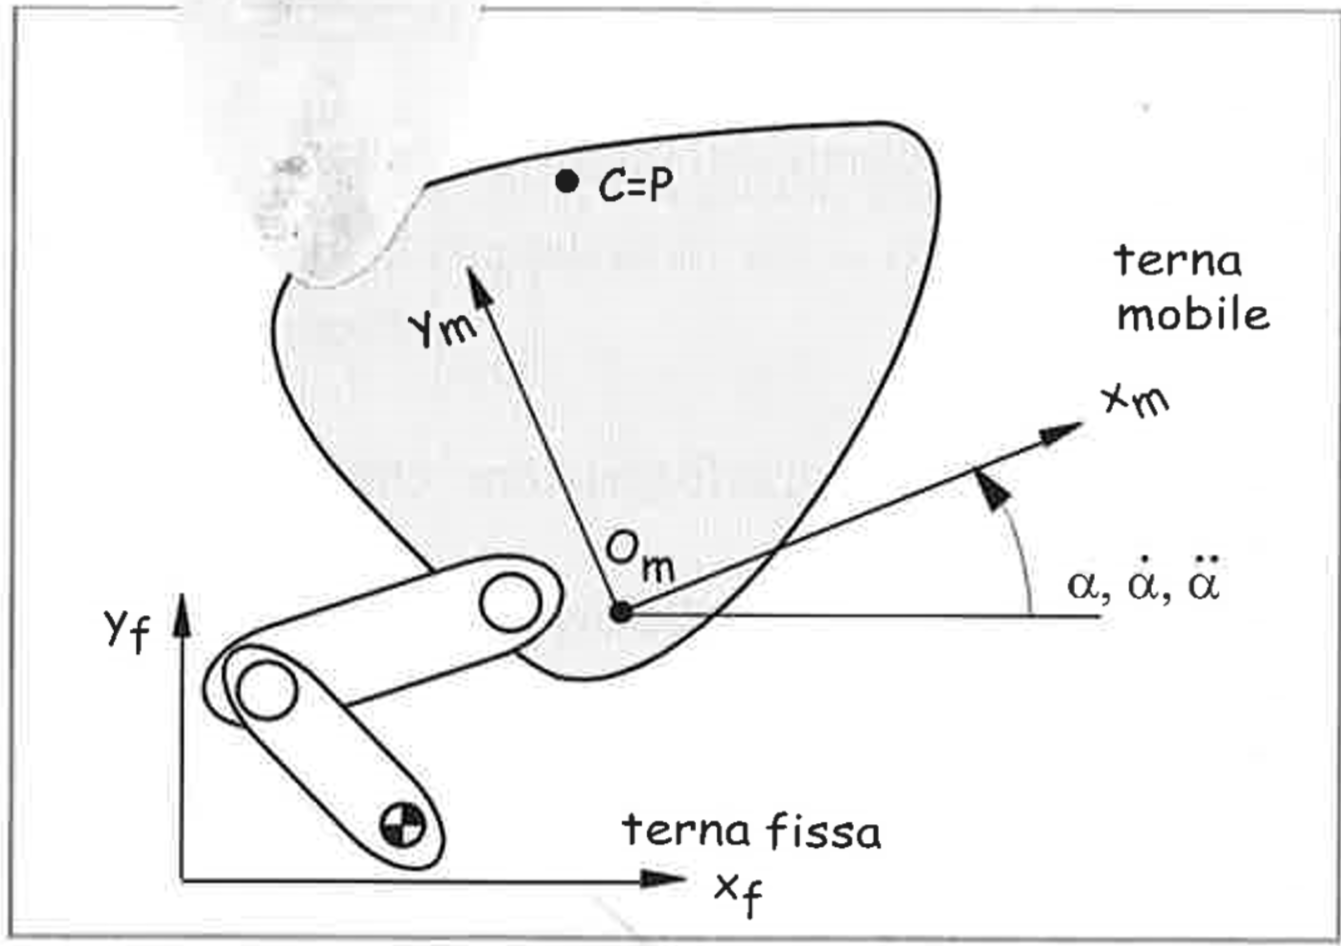
\includegraphics[width=.95\textwidth]{chapter03/Immagine212}
\end{minipage}
\vspace{1mm}

Imponiamo a P una velocità nulla e cerchiamo le due coordinate di P=C che soddisfano la relazione:
\[\leftidx{^f}{\B{\dot{x_C}\\\dot{y_C}}}=\leftidx{^f}{\B{0\\0}}=\leftidx{^f}{\B{\dot{x_{Om}}\\\dot{y_{Om}}}}\,+\,\dot{\alpha}\,\M{\cos{\alpha}&-\,\sin{\alpha}\\\sin{\alpha}&\cos{\alpha}}\,\leftidx{^m}{\B{-\,y_C\\x_C}}\]
da cui:
\[
\leftidx{^m}{\B{-\,y_C\\x_C}}=-\,\cfrac{1}{\dot{\alpha}}\,\,\leftidx{^m_f}{\M{R}}\,\leftidx{^f}{\B{\dot{x_{Om}}\\\dot{y_{Om}}}}
\]
ossia:
\begin{gather*}
^mx_C = \cfrac{^f\dot{x_{Om}}}{\dot{\alpha}}\,\sin{(\alpha)}\,-\,\cfrac{^f\dot{y_{Om}}}{\dot{\alpha}}\,\cos{(\alpha)}\qquad;\qquad^my_C = \cfrac{^f\dot{x_{Om}}}{\dot{\alpha}}\,\cos{(\alpha)}\,+\,\cfrac{^f\dot{y_{Om}}}{\dot{\alpha}}\,\sin{(\alpha)}
\end{gather*}
	
Il punto avente coordinate $^mx_C, ^my_C$ rispetto al sistema mobile viene chiamato centro di istantanea rotazione perché nell'istante considerato tutti i punti del corpo rigido ruotano attorno ad esso.

Le coordinate del centro di istantanea rotazione rispetto al sistema fisso \emph{f} si ottengono dalla trasformazione:
\[
\leftidx{^f}{\B{x_C\\y_C}}=\leftidx{^f}{\B{x_{Om}\\y_{Om}}}\,+\,\M{\cos{\alpha}&-\,\sin{\alpha}\\\sin{\alpha}&\cos{\alpha}}\,\leftidx{^m}{\B{x_C\\y_C}}=\leftidx{^f}{\B{x_{Om}\\y_{Om}}}\,+\,\M{\cos{\alpha}&-\,\sin{\alpha}\\\sin{\alpha}&\cos{\alpha}}\,\leftidx{^m}{\B{ \cfrac{^f\dot{x_{Om}}}{\dot{\alpha}}\,\sin{(\alpha)}\,-\,\cfrac{^f\dot{y_{Om}}}{\dot{\alpha}}\,\cos{(\alpha)}\\ \cfrac{^f\dot{x_{Om}}}{\dot{\alpha}}\,\cos{(\alpha)}\,+\,\cfrac{^f\dot{y_{Om}}}{\dot{\alpha}}\,\sin{(\alpha)}}}
\]
In definitiva si ottiene:
\begin{gather*}
^fx_C=^fx_{Om}\,-\,\cfrac{^f\dot{y_{Om}}}{\dot{\alpha}}\qquad;\qquad^fy_C=^fy_{Om}\,+\,\cfrac{^f\dot{x_{Om}}}{\dot{\alpha}}
\end{gather*}
Le formule che ci danno le coordinate del centro di istantanea rotazione mostrano che in generale esso si sposta sia nel sistema di riferimento mobile che nel sistema fisso. Il centro di istantanea rotazione non varia solo se il corpo ruota intorno ad un punto fisso.

Una volta noto il centro di istantanea rotazione si possono calcolare, in quell'istante, le velocità di tutti i punti del corpo rigido piano tramite la formula fondamentale dei corpi rigidi:

\begin{minipage}{.5\textwidth}
\[\mathbf{v_P}=\mathbf{v_C}\,+\,\und{\dot{\theta}}\,\wedge\,\mathbf{CP}\]
Poiché $\mathbf{v_C}$ è nulla si ottiene in forma scalare:
\[\B{\dot{x_P}\\\dot{y_P}}=\dot{\theta}\,\B{-\,CP_y\\CP_x}\]
Se invece in un istante la velocità angolare è nulla, tutti i punti del corpo rigido hanno la stessa velocità ed abbiamo quindi un moto traslatorio.
\end{minipage}
\hfill
\begin{minipage}{.5\textwidth}
\centering
\includegraphics[width=.7\textwidth]{chapter03/Immagine213}
\end{minipage}

In questo caso non esiste un centro di istantanea rotazione, infatti le due formule che permettono di calcolare il centro di istantanea rotazione hanno al denominatore la velocità angolare; se questa tende a zero, le coordinate del centro tendono all'infinito.

Possiamo ora enunciare il \textbf{teorema di Chasles}: le velocità dei punti di un corpo rigido nel moto piano o sono ortogonali alla congiungente i punti con il centro di istantanea rotazione (moto rotatorio) o sono parallele (moto traslatorio).

\begin{itemize}
\item \textbf{Esempio relativo ad un quadrilatero piano}
\end{itemize}

\begin{minipage}{.5\textwidth}
Vogliamo calcolare il centro di istantanea rotazione della biella 3 (non ruota attorno ad un asse fisso).

La velocità dei punti B e E sono già note.

B, che appartiene anche al segmento 2, ha velocità ortogonale al segmento AB mentre E, che appartiene al segmento 4, ha velocità ortogonale al segmento DE.

Ma la velocità di B, pensando B appartenente al segmento 3, deve essere, per il teorema di Chasles, ortogonale alla congiungente di B con il centro di istantanea rotazione di 3.

Per gli stessi motivi la velocità di E è ortogonale alla congiungente di E con il centro di istantanea rotazione di 3.

Perciò il centro di istantanea rotazione di 3 si trova all'intersezione tra la normale e $\mathbf{v_B}$, condotta per B e la normale a $\mathbf{v_E}$ condotta per E.
\end{minipage}
\hfill
\begin{minipage}{.5\textwidth}
\centering
\includegraphics[width=.95\textwidth]{chapter03/Immagine214}
\end{minipage}	

Tale centro, che è il centro di rotazione di 3 rispetto al segmento 1 (telaio) lo chiamiamo $C_{31}$.

Molto spesso non è sufficiente conoscere il centro di istantanea rotazione di un corpo rigido nel suo moto assoluto rispetto ad un sistema fisso, ma si deve conoscere il centro di rotazione di un corpo rigido nel so moto rispetto ad un altro corpo rigido in movimento.

Nel caso del quadrilatero ad esempio, si vuole conoscere il centro di istantanea rotazione di 4 rispetto a 2. Per calcolarlo possiamo pensare di sbloccare il membro 1 e di fissare a telaio il membro 2 e applicare la costruzione fatta precedentemente; in tal modo otteniamo il punto $C_{42}$, centro di istantanea rotazione di 4 rispetto a 2.

Gli altri centri di rotazione ($C_{12}, C_{23}, C_{34}, C_{41}$) sono tra segmenti contrigui e quindi coincidono con i centri delle coppie cinematiche.

Dalla figura osserviamo che i centri di istantanea rotazione sono a 3 a 3 allineati e ciò non è un caso.

Vale infatti il teorema di \textbf{Kennedy-Aronhold}: durante il moto rigido piano i centri di istantanea rotazione sono a 3 a 3 allineati. 

\subsection{Curve polari}

Abbiamo visto che in generale il centro di istantanea rotazione cambia in ogni istante. Perciò si sposta sia rispetto al sistema solidale al corpo rigido (di cui si studia il moto) che rispetto al sistema fisso.

Ad esempio nel quadrilatero il punto $C_{31}$ si muove sia rispetto alla biella che al telaio.

Chiamiamo polare fissa la traiettoria percorsa da C rispetto al membro fisso e polare mobile la traiettoria percorsa da C rispetto al membro mobile.

Vale il seguente teorema: durante il moto rigido la polare mobile rotola senza strisciare sulla polare fissa; durante il moto di rotolamento le due polari sono tangenti nel punto di contatto.

\begin{center}
\includegraphics[width=.7\textwidth]{chapter03/Immagine215}
\end{center}

\begin{itemize}
\item \textbf{Esempio di calcolo delle polari}
\end{itemize}

\begin{minipage}{.5\textwidth}
Consideriamo il meccanismo a crociera. Si voglia determinare la polare mobile e la polare fissa della biella AB.

Le coordinate e le velocità dell'origine della terna mobile rispetto al sistema fisso sono:
\begin{align*}
x_{Om}=0\qquad y_{Om}&=-\,l\,\sin{\alpha}\\
\dot{x_{Om}}=0\qquad \dot{y_{Om}}&=-\,\dot{\alpha}\,l\,\cos{\alpha}
\end{align*}
Da cui, applicando la formula che fornisce il centro di rotazione nel sistema fisso (polare fissa):
\begin{align*}
^fx_C&=^fx_{Om}\,-\,\cfrac{^f\dot{y_{Om}}}{\dot{\alpha}}&&^fx_C = l\,\cos{\alpha}\\
^fy_C&=^fy_{Om}\,+\,\cfrac{^f\dot{x_{Om}}}{\dot{\alpha}}&&^fy_C=-\,l\,\sin{\alpha}
\end{align*}
\end{minipage}
\hfill
\begin{minipage}{.5\textwidth}
\centering
\includegraphics[width=.95\textwidth]{chapter03/Immagine216}
\end{minipage}
\vspace{1mm}

Perciò al variare della configurazione del meccanismo (variazione di $\alpha$) il centro di istantanea rotazione descrive rispetto al sistema fisso una circonferenza di centro $O_f$ e raggio \emph{l}, questa è la polare fissa.

Di questo ci si poteva rendere conto anche graficamente dato che i punti A e B della biella hanno velocità sempre parallele rispettivamente all'asse y e x, le loro normali si incontrano nel punto C, che per il teorema di Chasles è centro di istantanea rotazione.

Il punto C appartiene al rettangolo $O_f$ABC che ha sempre diagonali uguali a \emph{l}, perciò la distanza di C da $O_f$ è sempre \emph{l} e quindi C si mantiene in una circonferenza.

Le coordinate del centro di istantanea rotazione nel sistema mobile sono (polare mobile):
\begin{align*}
^mx_C &= \cfrac{^f\dot{x_{Om}}}{\dot{\alpha}}\sin{\alpha}\,-\,\cfrac{^f\dot{y_{Om}}}{\dot{\alpha}}\cos{\alpha}&&^mx_C=l\,\cos^2{\alpha}=\cfrac{l}{2}(1\,+\,\cos{2\,\alpha})\\
^my_C &= \cfrac{^f\dot{x_{Om}}}{\dot{\alpha}}\cos{\alpha}\,+\,\cfrac{^f\dot{y_{Om}}}{\dot{\alpha}}\sin{\alpha}&&^my_C=-\,l\,\cos{\alpha}\,\sin{\alpha}=-\,\cfrac{l}{2}\,\sin{2\,\alpha}
\end{align*}

\begin{minipage}{.5\textwidth}
Perciò al variare della configurazione del meccanismo il centro di istantanea rotazione descrive rispetto al sistema mobile una circonferenza di raggio \emph{l}/2, avente origine (rispetto al sistema mobile) nel punto di coordinate (\emph{l}/2, 0). La polare mobile passa sempre per l'origine del sistema fisso perché è a contatto con la polare fissa nel punto C e ha diametro \emph{l}.

Ad esempio per $\alpha=45$° le coordinate del centro di istantanea rotazione risultano:
\begin{align*}
x_C&=0.707\,l&y_C&=-\,0.707\,l\\
^mx_C&=0.500\,l&^my_C&=-0.500\,l
\end{align*}
Se consideriamo il movimento relativo tra due membri ed entrambi sono mobili, allora anche il sistema di riferimento \emph{f} è mobile, le polari prendono in questo caso il nome di primitive
\end{minipage}
\hfill
\begin{minipage}{.5\textwidth}
\centering
\includegraphics[width=.9\textwidth]{chapter03/Immagine217}
\end{minipage}

\subsection{Profili coniugati}

\begin{minipage}{.6\textwidth}
Il moto di un membro mobile rispetto ad uno fisso è definito dal rotolamento della polare mobile sulla polare fissa.

Sia $\lambda_m$ una curva solidale al piano mobile diversa dalla polare mobile. Durante il moto rigido del piano mobile la curva $\lambda_m$ occupa sul piano fisso una infinità di posizioni che generalmente ammette ua curva inviluppo (tangente a $\lambda_m$ in tutte le posizioni) che chiamiamo $\lambda_f$.

Le due curve $\lambda_m$ e $\lambda_f$ si chiamano profili coniugati.

Valgono le seguenti importanti proprietà:
\end{minipage}
\hfill
\begin{minipage}{.4\textwidth}
\centering
\includegraphics[width=.95\textwidth]{chapter03/Immagine218}
\end{minipage}


\begin{enumerate}[$\rightarrow$]
\item Nel punto di contatto P i profili hanno tangente e normale comune
\item La normale comune passa per il centro di istantanea rotazione C.
\end{enumerate}

In generale tra i profili coniugati si ha strisciamento durante il moto relativo dei due membri, cioè velocità di strisciamento non nulla in P e diretta secondo la tangente.

Perciò il moto relativo tra due membri piani può essere definito, oltre che dal moto di puro rotolamento della polare mobile sulla polare fissa, anche dal moto con strisciamento di una coppia di profili coniugati, uno solidale al membro mobile e l'altro solidale al membro fisso. Questa è la soluzione comunemente adottata negli ingranaggi dove i profili coniugati sono i fianchi dei denti.

\begin{itemize}
\item \textbf{Esempio}
\end{itemize}

\begin{minipage}{.7\textwidth}
Consideriamo una coppia di ruote dentate, per comodità supponiamo che la ruota 1 sia fissata al telaio.

Cerchiamo il centro di istantanea rotazione $C_{21}$. Consideriamo due punti caratteristici del corpo 2 i punti B e P.

Il punto B, pensato appartenente al membro 3, ha velocità ortogonale alla retta AB; per il teorema di Chasles la retta AB deve quindi passare per il centro di istantanea rotazione.
\end{minipage}
\hfill
\begin{minipage}{.3\textwidth}
\centering
\includegraphics[width=.9\textwidth]{chapter03/Immagine219}
\end{minipage}

Il punto P, che è il punto di contatto tra i profili coniugati ha la velocità (velocità di strisciamento) allineata alla tangente comune ai due profili. Poiché la tangente è ortogonale alla normale ai profili, ne consegue che il centro di istantanea rotazione deve giacere sulla retta normale.

Il centro di istantanea rotazione è allora all'intersezione tra la retta AB e la normale in comune ai due profili.

Se ora andiamo a cosiderare il meccanismo che si ottiene tenendo fisso il membro 3, il punto $C_{21}$ rappresenta il centro di istantanea rotazione di 2 rispetto a 1; i tre centri sono allineati.